% based on a template made by the university of cologne
% http://www.mi.uni-koeln.de/wp-MIEDV/wp-content/uploads/2016/07/LaTeX-Vorlage.zip - 2023-11-02
\documentclass[12pt,a4paper]{scrartcl}

\addtokomafont{sectioning}{\rmfamily}
\usepackage[ngerman]{babel}% deutsches Sprachpaket wird geladen
\usepackage[T1]{fontenc} % westeuropäische Codierung wird verlangt
\usepackage[utf8]{inputenc}% Umlaute werden erlaubt
\usepackage[usenames]{color} % Erlaubt die Benutzung der namen im Farbpaket und deren Änderung
\usepackage{amsmath} % Erweiterung für den Mathe-Satz
\usepackage{amssymb} % alle Zeichen aus msam und msmb werden dargestellt
\usepackage{graphicx} % Graphiken und Bilder können eingebunden werden
\usepackage{multirow} % erlaubt in einer Spalte einer Tabelle die Felder in mehreren Zeilen zusammenzufassen
\usepackage{enumerate} % erlaubt Nummerierungen
\usepackage{xurl} % Dient zur Auszeichnung von URLs; setzt die Adresse in Schreibmaschinenschrift.
\usepackage[center]{caption}  % Bildunterschrift wird zentriert
%\usepackage{subfigure} % mehrere Bilder können in einer fugure-Umgebung verwendet werden
%\usepackage{longtable} % Diese Umgebung ist ähnlich definiert wie die tabular-Umgebung, erlaubt jedoch mehrseitige Tabellen.
%\usepackage{paralist} % Modifikation der bereits bestehenden Listenumgebungen
\usepackage{lmodern}% Für die Schrift
\usepackage[hidelinks]{hyperref} % Links und Verweise werden innerhalb von PDF Dokumenten erzeugt
%\usepackage{wrapfig} % Das Paket ermöglicht es von Schrift umflossene Bilder und Tabellen einzufügen.
\usepackage{latexsym} % LaTeX-Symbole werden geladen
\usepackage{tikz} % Erlaubt es mit tikz zu zeichnen
\usepackage{tabularx} % Erlaubt Tabellen
\usepackage{algorithm} % Erlaubt Pseudocode
\usepackage{color} % Farbpaket wird geladen
%\usepackage{stmaryrd} % St Mary Road Symbole werden geladen
\usepackage{physics}
\usepackage{mhchem} % Chemie: \ce & \pu

\numberwithin{equation}{section} % Nummerierungen der Gleichungen, die durch equation erstellt werden, sind gebunden an die section
\newcommand{\HRule}{\rule{\linewidth}{0.7mm}}
\newcommand{\pu}[1]{\ensuremath{\mathrm{#1}}}

\hyphenation{An-samm-lung }
\hyphenation{auf-wen-dig}
\hyphenation{Brems-me-di-ums}
\hyphenation{be-schreibt}
\hyphenation{Cu-rie-Tem-pe-ra-tur}
\hyphenation{Dop-pel-ätz-me-tho-de}
\hyphenation{ei-ner-seits}
\hyphenation{ein-ge-stellt}
\hyphenation{e-lek-tro-mag-ne-tische}
\hyphenation{Ener-gie-stragg-ling}
\hyphenation{Ent-mag-neti-sier-ungs-fak-tor}
\hyphenation{Ent-mag-neti-sier-ungs-feld-stär-ke}
\hyphenation{Ent-mag-neti-sier-ungs-ver-hal-ten}
\hyphenation{Erd-be-schleu-ni-gung}
\hyphenation{Er-eig-nis-se}
\hyphenation{er-kenn-bar}
\hyphenation{er-rei-chen}
\hyphenation{ge-ra-der}
\hyphenation{Ge-schoss-e-ner-gi-en}
\hyphenation{Ge-schwin-dig-keit}
\hyphenation{Grenz-be-reich}
\hyphenation{Koh-len-stoff-ket-ten}
\hyphenation{Kom-mu-tie-rungs-kur-ve}
\hyphenation{konn-te}
\hyphenation{kor-ri-gier-te}
\hyphenation{Li-te-ra-tur-wer-te}
\hyphenation{Li-thi-um-fluo-rid-Kris-tal-len}
\hyphenation{Mag-ne-ti-sier-ungs-aus-rich-tung}
\hyphenation{nach-ge-wie-sen}
\hyphenation{nächs-ten}
\hyphenation{nä-he-rungs-wei-se}
\hyphenation{Nor-mal-ver-tei-lung}
\hyphenation{or-ga-ni-schen}
\hyphenation{Pri-mär-elek-tron}
\hyphenation{Scha-len-mo-dells}
\hyphenation{Schnitt-flä-che}
\hyphenation{Se-kun-där-elek-tron-en}
\hyphenation{Se-kun-där-elek-tron-en-ver-viel-fach-er}
\hyphenation{statt-fin-det}
\hyphenation{sys-te-ma-tisch-en}
\hyphenation{Ver-ar-mungs-zo-ne}
\hyphenation{vi-su-a-li-siert}
\hyphenation{Wie-der-ho-lung}
\hyphenation{zu-sätz-lich}


\hypersetup{
  pdftitle={B3.4},
  pdfcreator={LaTeX via pandoc}}

\setcounter{secnumdepth}{6}
\setcounter{tocdepth}{6}

\begin{document}
\begin{titlepage}
	\pagestyle{empty}

	\begin{center}

	\textsc{\LARGE Universität zu Köln }\\ [0.4cm]
	\textsc{Mathematisch-Naturwissenschaftliche Fakultät} \\[1.5cm]

	
\includegraphics[width=0.45\textwidth]{../media/uni.jpg}\\[1.5cm]  % Uni-Logo wird geladen

	\textsc{\Large Praktikum~B}\\[2mm]
	\textsc{}\\[10mm]
	\HRule \\[0.4cm]

		{	\Huge \bfseries B3.4}\\[0.4cm]
			{	\huge \bfseries Positronen--Emissions--Tomographie}\\[0.3cm]
	
	\HRule \\[3cm]

 	\begin{center}
		\textsc{\Large Catherine~Tran } \\[3pt]
		\textsc{\Large Carlo~Kleefisch } \\[3pt]
		\textsc{\Large Oliver~Filla } \\[3pt]
	\end{center}
	\end{center}
\end{titlepage}

\newpage
\tableofcontents
\newpage

\hypertarget{einleitung}{%
\section{Einleitung}\label{einleitung}}

Die Positronen--Emissions--Tomographie (PET) ist ein nuklearmedizinisches bildgebendes Verfahren, bei denen radioaktive Materialien als \emph{Tracer} verabreicht werden, die dann im Körper des Patienten gemessen werden. Dadurch können Bilder von z.B. Krebszellen erzeugt werden.

In diesem Versuch wird eine radioaktive Quelle in einer Probe mittels der PET lokalisiert. Weiterhin wird die Ortsauflösung sowie die Winkelabhängigkeit untersucht.

\clearpage
\hypertarget{theoretische-grundlagen}{%
\section{Theoretische Grundlagen}\label{theoretische-grundlagen}}

\hypertarget{pet}{%
\subsection{PET}\label{pet}}
Die Positronen--Emissions--Tomographie ist ein Verfahren, das die Möglichkeit bietet, Veränderungen von Stoffwechselprozessen sowie physiologische Aktivitäten sichtbar zu machen. In der Medizin wird dieses Verfahren hauptsächlich verwendet, um Krebszellen im Körper zu detektieren.

Hierbei injiziert man dem Patienten radioaktive Markerstoffe, sogenannte \emph{Tracer}. Diese werden unterschiedlich von den Zellen aufgenommen und verarbeitet, abhängig vom lokalen Stoffwechsel. Damit der Körper nicht zu viel radioaktive Strahlungen ausgesetzt wird, muss der Tracer so kurzlebig sein, sodass dieser im Körper schnell zerfällt aber dennoch lang genug, um detektierbar zu sein. Zusätzlich muss er Positronen abgeben. Deswegen eignen sich z.B. $\ce{^{11}C}$, $\ce{^{13}N}$, $\ce{^{15}O}$, $\ce{^{18}F}$ besonders, die Halbwertzeiten hiervon sind zwischen $122,24 \,\mathrm s$ ($\ce{^{15}O}$) und $109,77\,\mathrm{min}$ ($\ce{^{18}F}$) \cite{NuclideChart}. Unterschiedliche Tracer werden für unterschiedliche Körperteile verwendet.

Wenn der Tracer im Gewebe ist, zerfällt er über den $\beta^+$--Zerfall und emittiert dabei Positronen. Innerhalb weniger Millimeter rekombiniert ein Positron mit einem Elektron und es kommt zur \emph{Paarvernichtung}. Hierbei entstehen zwei Photonen mit jeweils einer Energie von $\pu{511 \,keV}$ in einem Winkel von $180\,^\circ$ zueinander. \cite{Bethge,DGNM,Annihilation}

Um die Aktivität quantitativ zu bestimmen, werden Signale von den ausgestrahlten Photonen registriert. Wenn zwei davon koinzident sind, hat dieser Prozess mit großer Wahrscheinlichkeit auf der Verbindungslinie (LOR\footnote{Englisch: \emph{line of response}}) stattgefunden. Aus vielen solcher koinzidenten Signale lässt sich die Aktivität mit einem Computerprogramm zu einem zweidimensionalen und später dreidimensionalen Bild rekonstruieren.

Es kann bei der Messung häufig zu falschen Koinzidenzen kommen. Entweder sind das nur zufällige Signale, die zeitgleich aufgenommen werden, oder das Photon wurde schon auf den Weg zum Detektor gestreut. Diese falschen Koinzidenzen möchte man möglichst gering halten, da sie nicht zur Bildqualität beitragen und Nachbearbeitung fordern.

Neben der PET gibt es noch andere bildgebende Verfahren wie Röntgentomographie, Computertomographie (CT), Magnetresonanztomographie (MRT) und Ultraschall. Die Strahlenbelastung ist bei jeweiligem Verfahren unterschiedlich.

Bei Ultraschall werden nur unschädliche Schallwellen verwendet, sie werden von den Geweben, abhängig von der Struktur, unterschiedlich stark reflektiert, so können Bildkonstraste entstehen. MRT ist ebenso frei von Strahlenbelastung, durch ein starkes Magnetfeld richten sich die Wasserstoffkernspins alle in eine Richtung aus, aus dem Anteil der Spins lassen sich Gewebe voneinander unterscheiden.

Im Vergleich CT ist PET etwas weniger schädlich, da die Stoffe sehr schnell zerfallen. Die Strahlenbeslastung von PET entspricht ungefähr dem Doppelten bis Dreifachen der jährlichen natürlichen Belastung \cite{DGNM}, welche bei $\pu{2,1 \,mSv}$ pro Jahr liegt \cite{SSK}.

CT und Röntgentomographie nutzen energiereiche Röntgenstrahlungen und diese können das Erbgut schädigen. Dichte Gewebe wie Knochen lassen weniger Strahlungen durch als z.B Muskeln. Eine Röntgenaufnahme am Brustkorb hat eine Äquivalentdosis von $\pu{0,2 \,mSv}$ und eine CT am Brustkorb hat ca $\pu{8 \,mSv}$ \cite{SSK}.

Für die Medizin ist PET ein hervorragendes Werkzeug, besonders in der Onkologie. Das Verfahren kann Veränderung im Stoffwechsel erkennen, eher ein anderes Verfahren es nachweisen kann, so können Krebstumore früher erkannt und behandelt werden.

\hypertarget{betazerfall}{%
\subsection{\texorpdfstring{$\beta$--Zerfall}{\textbackslash beta--Zerfall}}\label{betazerfall}}

Der $\beta$--Zerfall ist eine der drei Arten radioaktiven Zerfalls. Wie beim $\alpha$--Zerfall wird dabei ein chemisches Element in ein anderes umgewandelt. Im Unterschied zum $\alpha$--Zerfall werden hierbei keine Nukleonen abgesondert, sondern ein Nukleon in ein anderes umgewandelt.

Es wird zwischen drei Arten des $\beta$--Zerfalls unterschieden. Es gibt $\beta^+$--Zerfall und $\beta^-$--Zerfall, weiterhin wird der Elektroneneinfang dazugezählt.

Radioaktiver Zerfall geschieht, wenn der Tochterkern eine höhere Bindungsenergie als der Mutterkern erhält. Es werden Neutronen benötigt, um die Coulombabstoßung \eqref{Coulombterm} der Protonen zu überwinden, jedoch verursachen zu viele Neutronen einen höheren Symmetrieterm in der Weizsäcker Massenformel \eqref{eq:Massenformel}. Daran kann man erklären, dass $\beta^-$--Zerfall dann geschehen kann, wenn der Kern zu viele Neutronen im Vergleich zu der Protonenanzahl hat.

Umgekehrt kann es zu $\beta^+$--Zerfall kommen, wenn der Kern nicht genügend Neutronen hat. Ebenso ist hierbei der Elektroneneinfang möglich. Welcher dieser Prozesse stattfindet hängt von der Energiedifferenz zwischen Mutterkern und Tochterkern ab: Wenn die Energiedifferenz kleiner als $\Delta E_\mathrm{min}=\pu{1,022\, MeV}$ beträgt, dann reicht die Energie nur für Elektroneneinfang. Bei einer Energie von mehr als $\Delta E_\mathrm{min}$ ist auch $\beta^+$--Zerfall möglich. $\Delta E_\mathrm{min}$ entspricht der doppelten Ruheenergie von Elektronen.

Beim $\beta^+$--Zerfall wird ein Proton $p$ in ein Neutron $n$ umgewandelt, dabei entstehen ein Positron $e^+$ sowie ein Elektronenneutrino $\nu_e$. Hierbei wird ein Mutterkern $\ce{^A_Z X}$ in einen Tochterkern $\ce{^A_{Z-1} Y^-}$ umgewandelt. Beim $\beta^-$--Zerfall wird ein Neutron $n$ in ein Proton $p$ umgewandelt, dabei entstehen ein Elektron $e^-$ sowie ein Elektronen--Antineutrino $\bar{\nu}_e$. Hierbei wird ein Mutterkern $\ce{^A_Z X}$ in einen Tochterkern $\ce{^A_{Z+1} Y^+}$ umgewandelt.

Beim Elektroneneinfang (ec) wird ähnlich wie beim $\beta^+$--Zerfall ein Proton $p$ in ein Neutron $n$ umgewandelt. Allerdings wird dazu ein Elektron $e^-$ verwendet, dass aus der $K$--Schale des Atoms eingefangen wurde. Daher wird nur ein Elektronenneutrino $\nu_e$ erzeugt. Hierbei wird ein Mutterkern $\ce{^A_Z X}$ in einen Tochterkern $\ce{^A_{Z-1} Y}$ umgewandelt.

\begin{eqnarray}
    \beta^+:\qquad\,\,\qquad
        \ce{p} &\ce{->}& \quad \ce{n} \quad\, + \ce{e^+} + \ce{\nu_e} \\
        \ce{^A_Z X} &\ce{->}& \ce{^A_{Z-1} Y^-} + \ce{e^+} + \ce{\nu_e} \\
    \beta^-:\qquad\,\,\qquad
        \ce{n} &\ce{->}& \quad \ce{p} \quad\, + \ce{e^-} + \ce{\bar{\nu}_e} \\
        \ce{^A_Z X} &\ce{->}& \ce{^A_{Z+1} Y^+} + \ce{e^-} + \ce{\bar{\nu}_e} \\
    \text{ec}:\qquad
        \ce{p + e^-} &\ce{->}& \quad \ce{n} \ \ \, + \ce{\nu_e} \\
        \ce{^A_Z X} &\ce{->}& \ce{^A_{Z-1} Y} + \ce{\nu_e}
\end{eqnarray}

\noindent
In diesem Versuch wird als Quelle $\ce{^{22}Na}$ verwendet, das eine Halbwertzeit von etwa 2,6 Jahren hat \cite{NuclideChart}. Dieses zerfällt über den $\beta^+$--Zerfall in einen angeregten Zustand des stabilen Isotops $\ce{^{22}Ne}$, welches unter Aussenden eines $\gamma$--Quants mit $E_\gamma = \pu{1275\, keV}$ in den Grundzustand zerfällt, siehe Abbildung \ref{abb:Skizze 22Na}. Beide Zerfälle geschehen koinzident.

\begin{figure}[h]
	\centering
	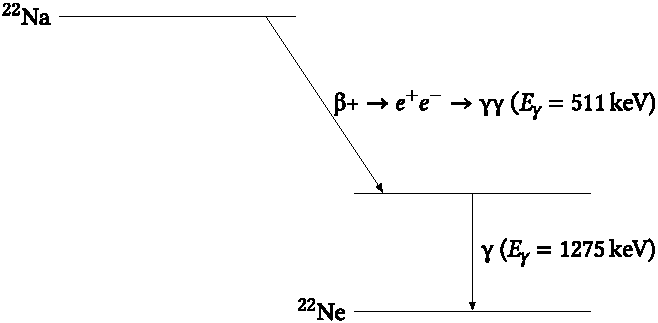
\includegraphics[width=0.7\textwidth]{../media/B3.4/Zerfall_22_Na.pdf}
	\caption{Skizze des Zerfalls von $\ce{^{22}Na}$ zu $\ce{^{22}Ne}$ \cite{UzK}}
	\label{abb:Skizze 22Na}
\end{figure}

\hypertarget{paarvernichtung}{%
\subsection{Paarvernichtung}\label{paarvernichtung}}

Der Begriff der Paarvernichtung beschreibt die Zerstrahlung von einem Teilchen und seinem Antiteilchen, bei der die Teilchen in $\gamma$--Strahlung umgewandelt werden. Die Energie der Strahlung ist die Summe der kinetischen Energie dieser Teilchen sowie ihrer Ruhemassen. Die Paarerzeugung ist der dazu inverse Effekt. \cite{Paarvernichtung}

Bei der Vernichtung eines Positrons $e^+$ mit einem Elektron $e^-$ entstehen normalerweise zwei $\gamma$--Quanten in einem Winkel $\theta$. Dieser hängt von der transversalen Impulskomponente $p_T$ ab. Weiterhin sind die Ruhemasse $m_e$ der Teilchen und die Lichtgeschwindigkeit $c$ relevant. \cite{Bethge,Annihilation}

\begin{eqnarray}
    \tan(\theta) &=& \frac{p_T}{m_ec}
\end{eqnarray}

\noindent
Sind die beiden Teilchen in Ruhe zueinander, so ist der Winkel der $\gamma$--Quanten $\pu{180\,^\circ}$. Dies liegt an der Impulserhaltung. Ist der Gesamtimpuls vor der Vernichtung $0$, so muss der Gesamtimpuls der beiden $\gamma$--Quanten ebenfalls $0$ sein.

Haben sie einen relativen Impuls, so wird der Winkel kleiner. Sind die Teilchen jedoch zu schnell, dann ist der Wirkungsquerschnitt sehr klein und es ist sehr unwahrscheinlich, dass Paarvernichtung stattfindet.

\hypertarget{gammastrahlung}{%
\subsection{\texorpdfstring{$\gamma$--Strahlung}{\textbackslash gamma--Strahlung}}\label{gammastrahlung}}

Gammastrahlung ist im engeren Sinne eine besonders durchdringende elektromagnetische Strahlung, die bei radioaktivem Zerfall auftritt. Sie wirkt durch drei Prozesse auf Materie. Bei einer Energie von bis zu $E_\gamma = \pu{100\, keV}$ überwiegt der Photoeffekt, weiterhin gibt es den Comptoneffekt und Paarbildung.

Für eine PET--Messung sind Comptoneffekt und Photoeffekt relevant. Die Energie der bei der Paarvernichtung erzeugten Gammaquanten ist zu niedrig, um Paarbildung zu verursachen. Daher sind der Comptoneffekt und der Photoeffekt relevant.

Aufgrund des sekundären Zerfalls bei der Abregung von $\ce{^{22}Ne}$ kann es in unserem Experiment auch zur Paarbildung kommen, da die Energie des hierbei erzeugten Gammaquants hoch genug ist.

Prinzipiell ist es dabei wahrscheinlich, dass nicht die gesamte Energie der $\gamma$--Strahlung im Detektor landet. Da dieser im  Unterschied zur umgebenden Luft eine sehr hohe Teilchendichte hat, ist es wahrscheinlich, dass ein Großteil der Wechselwirkungen im Detektor stattfinden. Bei hohem Luftdruck könnten die Wechselwirkungen mit der Luft dagegen deutlich größer werden.

\begin{figure}[h]
	\centering
	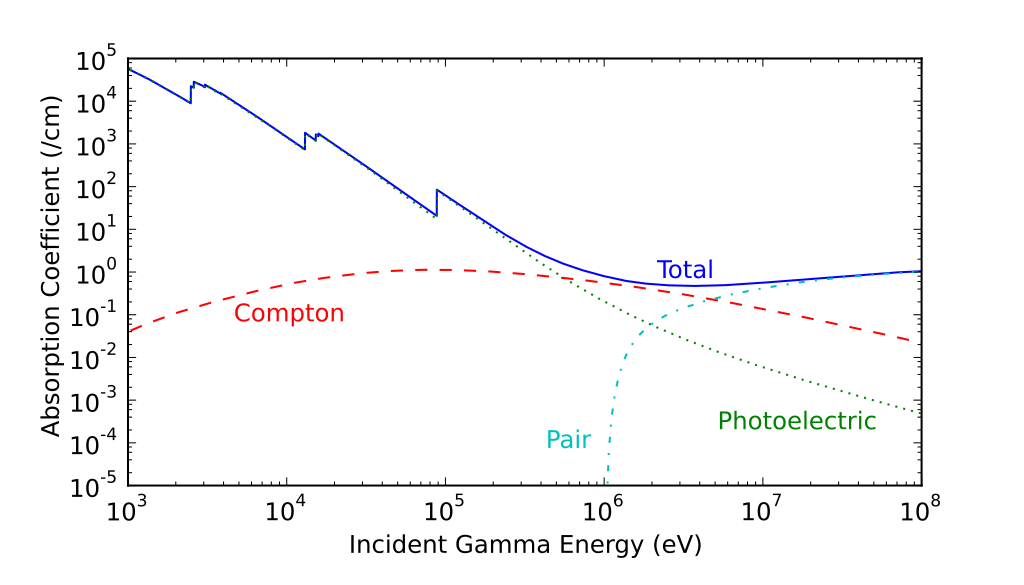
\includegraphics[width=0.9\textwidth]{../media/B3.4/1024px-Pb-gamma-xs.svg.png}
	\caption{Wirkungsquerschnitte von Photoeffekt (grün), Comptoneffekt (rot) und Paarbildung (türkis) \cite{abb:Wirkungsquerschnitte}}
	\label{fig:Wirkungsquerschnitte }
\end{figure}

\hypertarget{photoeffekt}{%
\subsubsection{Photoeffekt}\label{photoeffekt}}

Beim Photoeffekt überträgt ein Photon seine gesamte Energie auf ein Hüllenelektron, welches daraufhin das Atom verlässt. Er wirkt vor allem bei elektromagnetischer Strahlung mit einer Energie von bis zu $E_\gamma = \pu{100\, keV}$.

Die kinetische Energie $E_\mathrm{kin}$ des Elektrons hängt von der Energie des Photons $h\nu$ sowie der Austrittsarbeit $W_A$, ab. Letztere ist notwendig, um das Elektron aus dem Atom zu lösen.

\begin{eqnarray}
    E_\mathrm{kin} &=& h\nu - W_A
\end{eqnarray}

\noindent
Der Wirkungsquerschnitt $\sigma_\mathrm{ph}$ wird durch die Ordnungszahl $Z$, die reduzierte Photonenenergie $\epsilon$ $\eqref{redEnergie}$, die Sommerfeld'sche Feinstrukturkonstante $\alpha$ und den Thomson--\allowbreak Wirkungs-querschnitt $\sigma_\mathrm{Th}^e$ bestimmt. \cite{Bethge}

\begin{eqnarray}
    \sigma_\mathrm{ph}
        &=& \sqrt{\frac{32}{\epsilon^7}}\alpha^4 Z^5
            \sigma_\mathrm{Th}^e \pu{\,\frac{cm}{Atom}} \\
    \sigma_\mathrm{ph}
        &\propto& \frac{Z^5}{E_\gamma^{\frac{7}{2}}} \\
    \epsilon &=& \frac{E_\gamma}{m_ec^2} \label{redEnergie} \\
    \sigma_\mathrm{Th}^e &=& \frac{8}{3} \pi r_e^2
\end{eqnarray}

\noindent
Hierbei sind weiterhin die Elektronenmasse $m_e$ und der Radius $r_e$ eines Elektrons relevant.

Da die $\gamma$--Quanten in diesem Versuch im oberen Bereich dieses Energieintervalls liegen, wird der Photoeffekt in diesem Fall zur Ionisation der Atome führen.

\hypertarget{comptoneffekt}{%
\subsubsection{Comptoneffekt}\label{comptoneffekt}}

Der Comptoneffekt tritt vor allem bei $\gamma$--Strahlung mit mittleren Energien von ca. $\pu{100\, keV}$ bis $\pu{1\, MeV}$ auf. Dabei stößt ein Photon mit einem (quasi--freien) Elektron, wodurch es einen Impuls auf das Elektron überträgt und gestreut wird.

Die Änderung der Wellenlänge $\lambda$ des Photons hängt vom Streuwinkel $\theta$ ab. Der Wirkungsquerschnitt $\sigma_\mathrm{Co}$ ist von der Ordnungszahl $Z$ des Absorbers und der Energie $E_\gamma$ der Strahlung abhängig. \cite{Bethge}

\begin{eqnarray}
    \Delta \lambda &=& \frac{h}{m_e c} (1 - \cos(\theta)) \\
    \sigma_\mathrm{Co} &\propto & \frac{Z}{E_\gamma}
\end{eqnarray}

\noindent
Comptoneffekt und Photoeffekt unterscheiden sich in zwei Eigenschaften essenziell. Zum Einen wirkt der Photoeffekt nur auf gebundene, der Comptoneffekt dagegen auf quasifreie Elektronen. Zum Anderen wird beim Photoeffekt die gesamte Energie des Photons aufgebraucht, dagegen wird das Photon beim Comptoneffekt unter Energieverlust gestreut.

\hypertarget{paarbildung}{%
\subsubsection{Paarbildung}\label{paarbildung}}

Bei der Paarbildung entsteht aus einem Photon mit einer hohen Energie ein Teilchen--Antiteilchen--Paar, dieser Effekt dominiert bei Energien von etwa $\pu{5\, MeV}$. Die Umkehrung dieses Effektes nennt man Paarvernichtung.

Im Coulombfeld eines Atomkernes kann ein Photon zu einem Positron $e^+$ und einem Elektron $e^-$ zerstrahlen, wenn die Energie des Photons mindestens $\pu{1,022\, MeV}$ beträgt. Diese Energie entspricht der Gesamtmasse beider Teilchen.

Der Wirkungsquerschnitt $\sigma_\mathrm{Paar}$ kann wie folgt beschrieben werden. Wie bei dem Photoeffekt sind dabei die Feinstrukturkonstante $\alpha$ und der Elektronenradius $r_e$ relevant, ebenso die reduzierte Energie $\epsilon$ $\eqref{redEnergie}$.

\begin{eqnarray}
    \sigma_\mathrm{Paar}
        &=& 4\alpha r_e^2 Z^2
            \left(\frac{7}{9} \ln(2\epsilon) - \frac{109}{54} \right) \\
    \sigma_\mathrm{Paar}
        &\propto& Z^2 \ln(E_\gamma)
\end{eqnarray}

\hypertarget{impulshuxf6henspektrum}{%
\subsubsection{Impulshöhenspektrum}\label{impulshuxf6henspektrum}}

Die Zahl der in einem~Detektor~nachgewiesenen Ereignisse als Funktion ihrer Impulshöhe wird durch ein Impulshöhenspektrum dargestellt, was in Abbildung \ref{abb:Impulshoehenspektrum} zu sehen ist. \cite{Impulshöhenspektrum}

\begin{figure}[h]
	\centering
	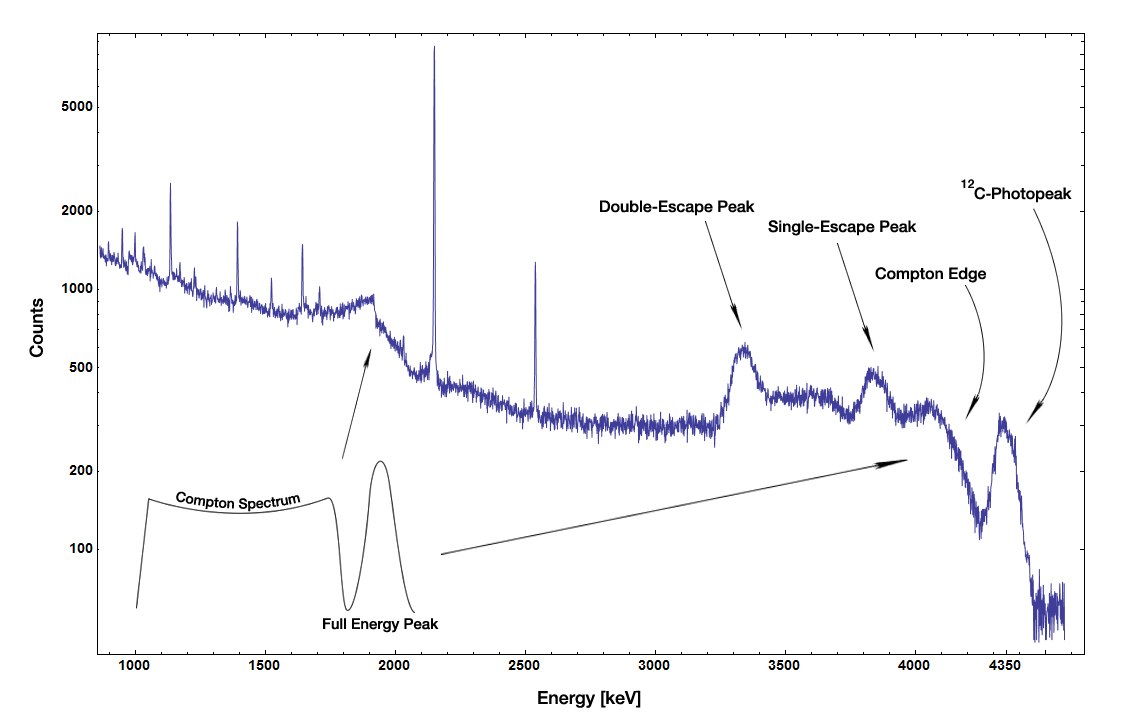
\includegraphics[width=0.9\textwidth]{../media/B3.4/Am_Be_SourceSpectrum.jpg}
	\caption{Impulshöhenspektrum für \\
		monoenergetische Gamma--Übergänge in $\ce{^{24}Mg}$  \cite{abb:Spektrum}}
	\label{abb:Impulshoehenspektrum}
\end{figure}

\paragraph{Photopeak}

Ein Photopeak (\emph{Full--Energy--Peak}) entsteht, wenn die gesamte Energie eines Photons in einem Detektor gemessen wird. Dies ist dann der Fall, wenn das Photon vor dem Eintreten in den Detektor keine Energie durch Wechselwirkungen verloren hat. Dann kann das Photon seine Energie über den Comptoneffekt und den Photoeffekt im Detektor deponieren.

\paragraph{Compton--Kante}

Werden viele Photonen mit der gleichen Energie durch den Comptoneffekt gestreut, so ergibt sich ein charakteristisches Energiespektrum der gestreuten Elektronen, siehe Abbildung \ref{abb:Compton-Kante}. Die hierbei auf die Elektronen übertragene Energie ist eine kontinuierliche Funktion des Streuwinkels~$\phi$, hat jedoch eine scharfe obere Schranke.

\begin{figure}[h]
	\centering
	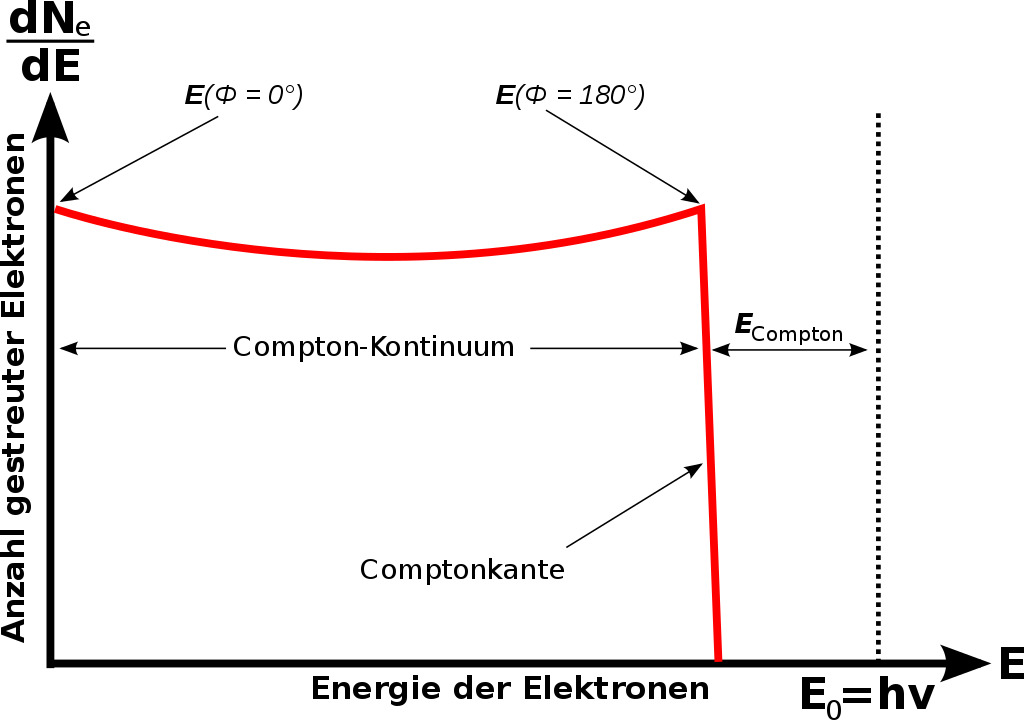
\includegraphics[width=0.7\textwidth]{../media/B3.4/Comptonspektrum.jpg}
	\caption{Compton--Kontinuum und Compton--Kante \cite{abb:Compton}}
	\label{abb:Compton-Kante}
\end{figure}

Das Compton--Kontinuum $E_e'(\phi)$ beschreibt den Energie des Elektrons nach dem Stoß $\eqref{Compton--Kontinuum}$, die obere Schranke derselben ist die \emph{Compton--Kante} $E_e(180^\circ)$ $\eqref{Compton--Kante}$. Die Energie des Photons nach der Streuung $E_{\gamma}^\prime(\phi)$ wird dagegen durch die Klein--Nishina--Formel $\eqref{Klein--Nishina}$ beschrieben.

\begin{eqnarray}
    E_e^\prime(\phi)
        &=& E_{\gamma} - E_{\gamma}'(\phi) \\
        &=& E_{\gamma}
            \left(
                1-
                \frac{1}{1+\frac{E_{\gamma}}{m_\mathrm ec^2}
                    (1-\cos(\phi))}
            \right) \label{Compton--Kontinuum} \\
    E_e^\prime(180^\circ) &=& \frac{E_\gamma}{1+\frac{m_ec^2}{2E_\gamma}}
        \label{Compton--Kante} \\
    E_{\gamma}^\prime(\phi)
        &=& \frac{E_{\gamma}}{1+\frac{E_{\gamma}}{m_\mathrm ec^2}
            (1-\cos\phi)} \label{Klein--Nishina}
\end{eqnarray}

\paragraph{Rückstreupeak}

Ein Compton--Rückstreuungspeak (\emph{Backscatter Peak})~tritt bei der Energie $E_\mathrm{Rück}$ auf, wenn die $\gamma$--Strahlen in das Material um den Detektor herum gestreut wurden und erst danach in den
den Detektor treffen. \cite{Bethge}

\begin{eqnarray}
    E_\mathrm{Rück} &=& E_\gamma - E_e^\prime(180^\circ)
\end{eqnarray}

\paragraph{Escapelinien}

Escapelinien oder Escape--Peaks sind unechte Spektrallinien, die bei der Röntgen- und Gammaspektroskopie auftreten und z.B. die Anwesenheit nicht vorhandener Radionuklide in der gemessenen Probe vortäuschen können. \cite{Escapelinie}

Gammastrahlung mit einer Energie von $E_\gamma\ge\pu{1022\,MeV}$ kann zur Paarbildung führen. Dabei entstehende Positronen zerstrahlen wiederum mit anderen Elektronen. Dies kann auch in einem Detektor geschehen. Es ist dabei nicht garantiert, dass die dabei entstehenden $\gamma$--Quanten detektiert werden. \cite{Bethge}

Wenn nur ein Photon detektiert wird, verursacht dies einen \emph{Single--Escape--Peak} bei einer Energie von
$E_\gamma - \pu{511\, keV}$. Wird keines der Photonen detektiert, gibt es einen \emph{Double--Escape--Peak} bei der Energie $E_\gamma - \pu{1022\, keV}$.

\hypertarget{weizsuxe4cker-massenformel}{%
	\subsubsection{Weizsäcker Massenformel}\label{weizsuxe4cker-massenformel}}
Die \emph{Weizsäcker Formel} gibt die Bindungsenergie eines Atomkerns an. Sie basiert einerseits auf empirischen Daten, andererseits auf dem Tröpfchenmodell. Aus ihr wird die Weizsäcker Massenformel ermittelt.

Das Tröpfchenmodell beschreibt einen Atomkern als einen inkompressiblen, kugelförmigen Fluidtropfen, der zur Energieminimierung den Kernradius $R$ aufweist. Dabei ist die Dichte überall konstant.

Die Bindungsenergie $E_B$ wird aus fünf verschiedenen Termen ermittelt, auf die im Folgenden eingegangen wird. Diese Terme werden durch die empirisch ermittelten Faktoren $a_i$ sowie die Nukleonenzahl bzw. Massenzahl $A$, Protonenzahl $Z$ und Neutronenzahl $N$ beschrieben. Hierbei handelt es sich um den Volumenterm $E_V$ $\eqref{Volumenterm}$, den Oberflächenterm $E_O$ $\eqref{Oberflächenterm}$, den Coulombterm $E_C$ $\eqref{Coulombterm}$, den Symmetrieterm $E_S$ $\eqref{Symmetrieterm}$ und den Paarungsterm $E_P$ $\eqref{Paarungsterm}$.

\begin{eqnarray}
	E_B &=& E_V + E_O + E_C + E_S + E_P
\end{eqnarray}

\noindent
Die Bindungsenergie $E_B$ verringert die Masse des Atomkernes. Daher kann die Kernmasse $m$ durch die Protonenmasse $m_P$, die Neutronenmasse $n_N$ sowie $E_B$ beschrieben werden, wobei die Lichtgeschwindigkeit $c$ die Energie in Masse konvertiert. Dies ergibt die \emph{Weizsäcker Massenformel}.

\begin{eqnarray}
	m &=& N\cdot m_N + P\cdot m_P - \frac{E_B}{c^2} \label{eq:Massenformel}
\end{eqnarray}

\noindent
In der Darstellung der einzelnen Terme ist weiterhin relevant, dass der Kernradius $R$ durch den Radius $r$ eines Nukleons und die Nukleonenzahl $A$ beschrieben werden kann.

\begin{eqnarray}
	R &=& r \cdot \sqrt[3]{A}
\end{eqnarray}

\hypertarget{volumenterm}{%
	\paragraph{Volumenterm}\label{volumenterm}}

Der Volumenterm $E_V$ beschreibt die Anziehung der Nukleonen durch die starke Wechselwirkung.

Diese hat eine Reichweite von $2,5\mathrm{\,fm}$, weswegen sie nur auf die nächsten Nachbarn eines Nukleons wirkt. Da die Dichte im Kern nach dem Tröpfchenmodell konstant ist, ist die gesamte Bindungsenergie durch die starke Wechselwirkung proportional zum Kernvolumen. Dieses wiederum ist proportional zu $R^3\propto A$.

\begin{eqnarray}
	E_V &=& + a_V\cdot A \label{Volumenterm} \\
	a_V &=& 15,85\mathrm{\,MeV}
\end{eqnarray}

\hypertarget{oberfluxe4chenterm}{%
	\paragraph{Oberflächenterm}\label{oberfluxe4chenterm}}

Da die Atome an der Oberfläche des Atomkerns weniger Nachbarn haben als die Nukleonen im Kern, wird sind die ersteren schwächer gebunden. Daher beschreibt der Oberflächenterm $E_O$ eine Korrektur des Volumenterms. Diese ist proportional zur Oberfläche einer Kugel mit dem Kernradius $R$, also proportional zu $\sqrt[3]{A^2}$.

\begin{eqnarray}
	E_O &=& - a_O\cdot \sqrt[3]{A^2} \label{Oberflächenterm} \\
	a_O &=& 18,34\mathrm{\,MeV}
\end{eqnarray}

\hypertarget{coulombterm}{%
	\paragraph{Coulombterm}\label{coulombterm}}

Der Coulombterm $E_C$ beschreibt die elektrostatische Abstoßung der Protonen voneinander, die die Bindungsenergie senkt. Jedes der $Z$ Protonen wird von den anderen $(Z-1)$ Protonen abgestoßen. Die Coulombwechselwirkung ist proportional zu $R^{-1}\propto\left(\sqrt[3]{A}\right)^{-1}$.

\begin{eqnarray}
	E_C &=& - a_C\cdot \frac{Z(Z-1)}{\sqrt[3]{A}} \label{Coulombterm} \\
	a_C &=& 0,71\mathrm{\,MeV}
\end{eqnarray}

\noindent
Für große Kerne mit $Z\approx(Z-1)$ kann der Term $Z(Z-1)\approx Z^2$ vereinfacht werden.

\hypertarget{symmetrieterm}{%
	\paragraph{Symmetrieterm}\label{symmetrieterm}}

Der Symmetrieterm $E_S$ beschreibt die Verringerung der Bindungsenergie durch ein Ungleichgewicht von Protonen und Neutronen.

Die Ursache kann quantenmechanisch erklärt werden. Protonen und Neutronen werden als Fermigas in einem Potentialtopf betrachtet. Beide Gase teilen sich denselben Potentialtopf und füllen Einteilchenniveaus bis zu ihrer jeweiligen Fermienergie auf. Sind genau gleich viele beider Teilchensorten vorhanden, so sind alle Zustände bis zur Fermienergie besetzt.

Gibt es jedoch ein Teilchen mehr von einer Sorte, so müssen höhere Energieniveaus besetzt werden. Sei z.B. ein Proton mehr vorhanden, so muss ein Proton ein höheres Energieniveau als alle anderen Nukleonen besetzen. Dies benötigt mehr Energie.

Wandelt man nun in einem symmetrischen Kern ein Nukleon um, so erhöht man die eine Fermienergie und senkt die andere ab. Dieser Prozess kostet Energie, der Betrag der Energie ist die Differenz zwischen den Ferminiveaus. Wenn man die Energiedifferenz in einer Tabelle aufträgt, sieht man, dass der Term erst am Anfang mit $(N-Z)$ wächst und bei Umschichtungen von drei Nukleonen eine besser Beschreibung das Wachstum mit $(N-Z)/2$ ist. Wenn man dann noch betrachtet, dass Abstand der Einteilchenniveaus mit steigendem Volumen sinkt, erhält man mit der Proportionalität zwischen Volumen und Nukleonenzahl $A$ folgende Formel.

\begin{eqnarray}
	E_S &=& - a_S\cdot \frac{(N-Z)^2}{4A} \label{Symmetrieterm} \\
	a_S &=& 2,86\mathrm{\,MeV}
\end{eqnarray}

\hypertarget{paarungsterm}{%
	\paragraph{Paarungsterm}\label{paarungsterm}}

Der Paarungsterm $E_P$ beschreibt das Phänomen, dass gerade Anzahlen von Protonen bzw. Neutronen in einem Kern stabilere Kerne produzieren. Paare von Protonen oder Neutronen sind stärker gebunden als ein ungepaartes Proton oder Neutron.

Deswegen wird zwischen $\mathrm{gerade}$--$\mathrm{gerade}$--Kernen $(\mathrm{gg})$, $\mathrm{gerade}$--$\mathrm{ungerade}$--Kernen $(\mathrm{gu})$ und $\mathrm{ungerade}$--$\mathrm{gerade}$--Kernen $(\mathrm{ug})$ sowie $\mathrm{ungerade}$--$\mathrm{ungerade}$--Kernen $(\mathrm{uu})$ unterschieden. Erstere haben jeweils eine gerade Anzahl von Protonen und Neutronen, während letztere jeweils ungerade Anzahlen haben. $\mathrm{ug}$-- und $\mathrm{gu}$--Kerne haben eine Nukleonensorte in gerader und die andere in ungerader Menge.

Bei einer geraden Anzahl derselben Nukleonensorte heben sich die Spins auf, bei einer ungeraden Anzahl nicht. Auf diese Weise kann das Phänomen mithilfe des Schalenmodells erklärt werden.

Der Paarungsterm wird betragsmäßig kleiner, je größer die Nukleonenzahl $A$ ist. Dies wird durch die folgende Gleichung beschrieben.

\begin{eqnarray}
	E_P &=&
	\begin{cases}
		+ a_P\cdot \frac{1}{\sqrt{A}} & \text{gg} \\
		0 & \text{gu} \\
		0 & \text{ug} \\
		- a_P\cdot \frac{1}{\sqrt{A}} & \text{uu} \\
	\end{cases}
	\label{Paarungsterm} \\
	a_P &=& 11,46\mathrm{\,MeV}
\end{eqnarray}

\noindent
Beide Nukleonensorten liefern betragsmäßig den gleichen Beitrag zu $E_P$. Bei $\mathrm{gg}$-- und $\mathrm{uu}$--Kernen addieren sich diese Werte zu einer nicht--verschwindenden Energie. Bei $\mathrm{gu}$-- und $\mathrm{ug}$--Kernen heben sich die Terme dagegen auf, weswegen der Paarungsterm hier verschwindet.

\hypertarget{elektronik}{%
\subsection{Elektronik}\label{elektronik}}

In diesem Versuch werden verschiedene elektronische Bauteile verwendet, die im Folgenden näher erläutert werden. In \ref{abb:Schaltplan} ist eine Schaltskizze des Versuchs zu finden.

Als Detektor für die koinzidenten Signale werden anorganische Szintillationszähler sowie Photomultiplier zur Elektronenvervielfachung verwendet.

In diesem Versuch wird $\ce{NaI}$ als anorganischer Szintillator verwendet. Dieser wird oft mit Thalium dotiert, hierbei beträgt die Lichtausbeute etwa $10\,\%$ \cite{EigenschaftenSzintillatoren}.

\begin{figure}[h]
	\centering
	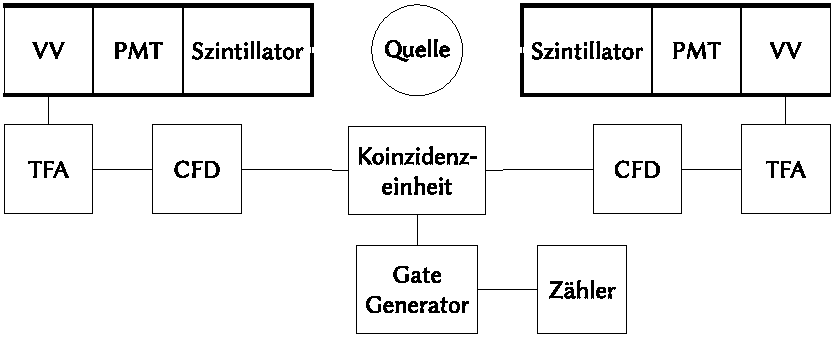
\includegraphics[width=0.7\textwidth]{../media/B3.4/Schaltplan.pdf}
	\caption{Schaltskizze des Versuchs, bestehend aus
		Photomultiplier (PMT), Vorverstärker (VV),
		Hauptverstärker (TFA) und Diskriminator (CFD) \cite{UzK}}
	\label{abb:Schaltplan}
\end{figure}


\hypertarget{verstuxe4rker}{%
\subsubsection{Verstärker}\label{verstuxe4rker}}

Ein Verstärker wird dazu verwendet ein eintreffendes elektronisches Signal zu verstärken. Dabei wird zwischen Vor- und Hauptverstärker unterschieden.

Ein Vorverstärker wird direkt an die Detektoren angeschlossen, oder die Detektoren haben, wie in diesem Versuch, bereits einen Vorverstärker integriert. Dieser dient dazu, das von den Detektoren stammende Signal
zu verstärken, sodass die Verluste in den Kabeln, die den Detektor mit den anderen Bauteilen verbinden, minimiert werden.

Der in diesem Versuch verwendete Hauptverstärker, ein \emph{Timing Filter Amplifier} (TFA), dient dazu, dem Signal eine möglichst kurze Anstiegsflanke zu verleihen. Er empfängt das Signal aus den Vorverstärkern, verstärkt es und leitet es weiter zu den Diskriminatoren.

Alternativ kann man einen \emph{Spectroscopy Amplifier} (SA) als Hauptverstärker nutzen, der das Signal möglichst verzerrungsfrei verstärkt. Dies ist für Messungen interessant, in denen die Energieauflösung wichtiger als die Zeitauflösung ist.

\hypertarget{diskriminator}{%
\subsubsection{Diskriminator}\label{diskriminator}}

Ein Diskriminator ist ein Bauteil, das ein logisches Signal\footnote{Ein logisches Signal ist ein Kastensignal, das nur zwei verschiedene Werte annimmt.} einer gewissen Breite ausgibt, falls die Amplitude des eintreffenden Signals eine einstellbare Schwelle überschreitet.

Da in diesem Versuch die Messung von zwei koinzidenten $\gamma$--Quanten relevant ist, ist es wichtig, dass die Diskriminatoren die logischen Signale zweier zeitgleich eintreffenden Signale auch zeitgleich ausgeben. Dabei gibt es jedoch zwei Probleme, den \emph{Walk} und den \emph{Jitter}.

\paragraph{Walk}
Treffen zwei Signale zeitgleich in zwei Detektoren ein, haben aber unterschiedliche maximale Amplituden, erreichen diese beiden Signale die Amplituden--Schwelle der Diskriminatoren zu unterschiedlichen Zeitpunkten. Dies ist in Abbildung \ref{abb:Walk-Effekt} dargestellt.

Die von den Diskriminatoren ausgesendeten logischen Signale sind dadurch zeitverschoben, obwohl die eintreffenden Signale koinzident waren. Diese Verschiebung der logischen Signale wird \emph{Walk} genannt.

\begin{figure}[h]
	\centering
	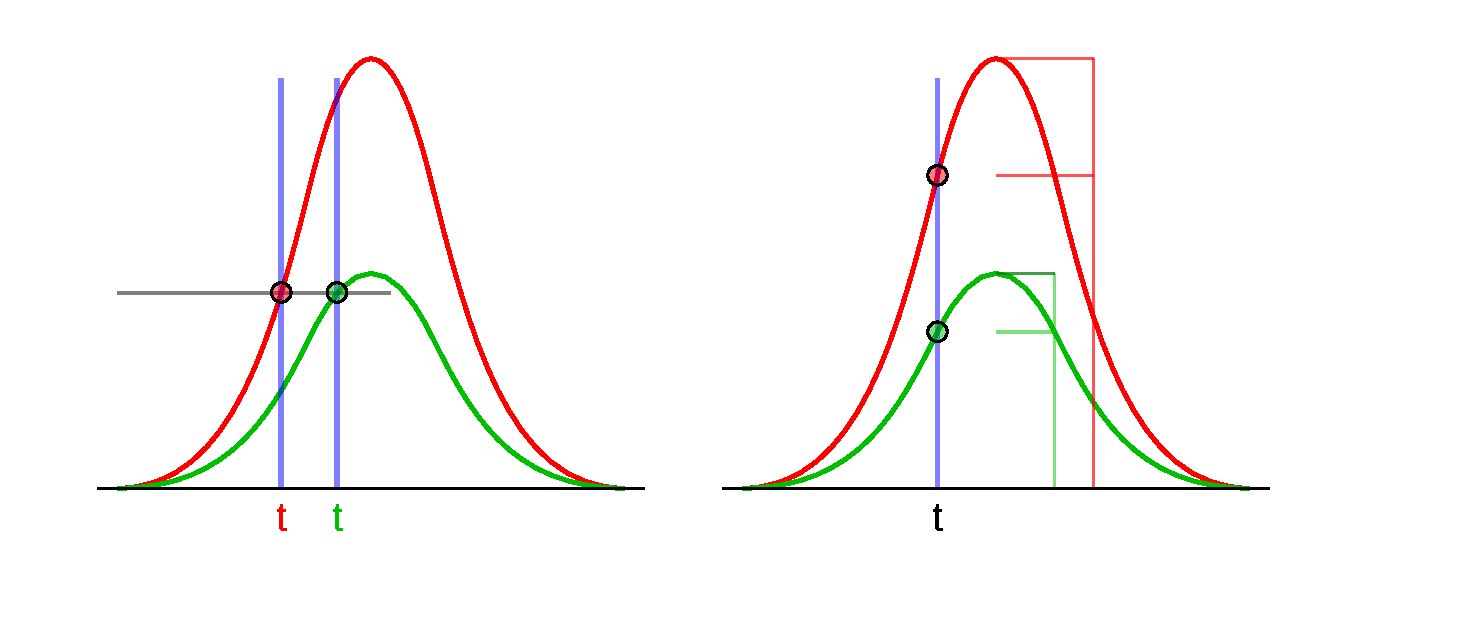
\includegraphics[width=0.7\textwidth]{../media/B3.4/Constant_fraction_1.pdf}
	\caption{Links: Walk--Effekt, Rechts: Kein Walk--Effekt \cite{abb:Constant_fraction}}
	\label{abb:Walk-Effekt}
\end{figure}

\hypertarget{jitter}{%
\paragraph{Jitter}\label{jitter}}

Aufgrund von statistischen Fluktuationen und Untergrundrauschen \allowbreak kann es passieren, dass zwei eigentlich gleiche Signale einen unterschiedlichen Zeitverlauf aufweisen. Daraufhin kann sich wie schon beim Walk der Zeitpunkt unterscheiden, bei dem die Signale die Amplituden--Schwelle der Diskriminatoren erreichen, wodurch die ausgesendeten logischen Signale wieder zeitversetzt sind. Dieses Phänomen wird als \emph{Jitter} bezeichnet.

\hypertarget{cfd}{%
\paragraph{Constant--Fraction--Diskriminator}\label{cfd}}

Um den Problemen durch Walk und Jitter entgegenzuwirken, wird in diesem Versuch ein \emph{Constant--Fraction--Diskriminator} (CFD) verwendet. Ein CFD teilt ein eintreffendes Signal in zwei Teilsignale. Das erste Teilsignal wird um eine gewisse Zeit $T$ verzögert. Das zweite Teilsignal wird invertiert und um einen Faktor $k\in(0, 1)$ gestaucht. Daraufhin werden beide Teilsignale wieder addiert. Der CFD sendet das logische Signal dann erst aus, wenn das wie oben beschrieben veränderte Signal seinen Nulldurchgang erreicht. Es ist in Abbildung \ref{abb:CFD} dargestellt.

\begin{figure}[h]
	\centering
	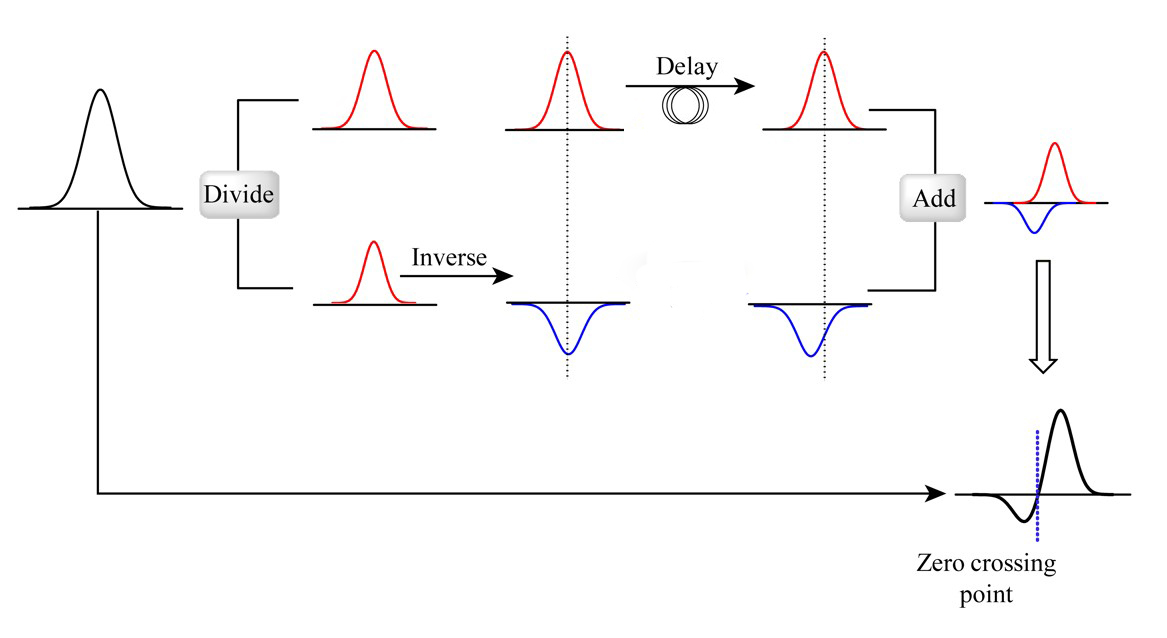
\includegraphics[width=0.7\textwidth]{../media/B3.4/CFD.jpg}
	\caption{Funktionsprinzips eines Constant--Fraction--Diskriminators \cite{abb:CDF}}
	\label{abb:CFD}
\end{figure}

\hypertarget{koinzidenzeinheit}{%
\subsubsection{Koinzidenzeinheit}\label{koinzidenzeinheit}}

Die logischen Signale aus den beiden Diskriminatoren werden dann gemeinsam zur Koinzidenzeinheit weitergeleitet. Diese überprüft, ob sich die beiden Signale überlappen. Falls dies der Fall ist, sendet sie ein logisches Signal an einen \emph{Gate Generator}, der das Signal in ein genormtes logisches Signal umformt. Dieses wiederum wird an den Zähler weitergegeben.

\hypertarget{szintillatoren}{%
\subsubsection{Szintillatoren}\label{szintillatoren}}
Wenn Photonen auf ein Szintillationsmaterial treffen, wechselwirken sie und regen die Elektronen an. Nach einer Zeit fallen diese wieder in den Grundzustand ab und senden dabei Licht im sichtbaren Bereich aus. Die Zeit dieses Ablaufs beträgt abhängig vom verwendeten Material zwischen $\pu{100\, ps}$ und $\pu{1\,\mu s}$.

Wenn Photonen auf den Szintillationskristall treffen, wird die Energie des Photons auf Elektronen im Valenzband übertragen und die Elektronen werden ins Leitungsband angehoben. Fallen sie wieder zurück ins Valenzband, wird erneut ein Photon mit derselben Energie emittiert. Mit sehr hoher Wahrscheinlichkeit wird dieses Photons wieder direkt von einem anderen Elektron im Valenzband absorbiert, dies kann unendlich oft passieren.

Um diesem endlosen Effekt entgegenzuwirken dotiert man den Kristall so, dass die Bandlücke lokal durch Energiezustände von diesen Atomen verkleinert wird. Die Elektronen können dann in verschiedene Zuständen zwischen Valenz- und Leitungsband fallen und emittieren dabei Photonen im sichtbaren Bereich. Diese Photonen haben aber nicht mehr die Größe der vorherrschenden Bandlücke und werden daher auch nicht wieder absorbiert.

Diese Photonen treffen dann auf die Kathode des Photomultipliers, welcher im nächsten Kapitel erläutert wird.

Häufig sind Szintillatoren anorganische Isolatoren oder Halbleiter mit einer großen Bandlücke. Der Vorteil von anorganischen Szintillatoren aus Kristall oder Glas ist die hohe Lichtausbeute, welche sehr wichtig für die Energiemessgenauigkeit ist. Nachteilig dagegen ist die langsame Lichtemission im Bereich von einigen $\pu{100\, ns}$, die Energieauflösung sowie die Feuchtigkeitsempfindlichkeit von manchen Kristallen.

Ein Photon aus einem Paarvernichtungsprozess mit einer Energie von $\pu{511\,keV}$ kann zehntausende Elektronen anregen, da diese mit Energien im $\pu{eV}$--Bereich gebunden sind. Beim Wasserstoff ist das Elektron mit $\pu{13,6\,eV}$ gebunden, hier könnten theoretisch bis zu $35,6\cdot 10^3$ Photonen angeregt werden.

Weiterhin gibt es organische Szintillatoren, die haupsächlich aus langen Kohlenstoffketten bestehen. Das Licht wird durch zwei Hauptprozesse erzeugt, die Floureszenz und die Phosphoreszenz. \cite{LMU}

Floureszenz ist ein Prozess, bei dem ein absorbiertes Photon nach Anregung sofort wieder abgestrahlt wird, dies erfolgt durch einen erlaubten Übergang zwischen zwei Zuständen. \cite{LMU}

Der Prozess der Phosphoreszenz läuft dagegen langsamer ab, weil ein verbotener Übergang zwischen einem angeregten Zustand und dem Grundzustand durch eine Multipol--Auswahlregel stattfinden muss. Im Allgemeinen kommt das Lichtsignal in einem organischen Szintillator früher als im anorganischen, im Idealfall kommt es schon nach $\pu{100\, ps}$. Trotz diesem Vorteil haben sie nur eine geringe Lichtausbeute. \cite{LMU}

\hypertarget{photomultiplier}{%
\subsubsection{Photomultiplier}\label{photomultiplier}}

\begin{figure}[h]
	\centering
	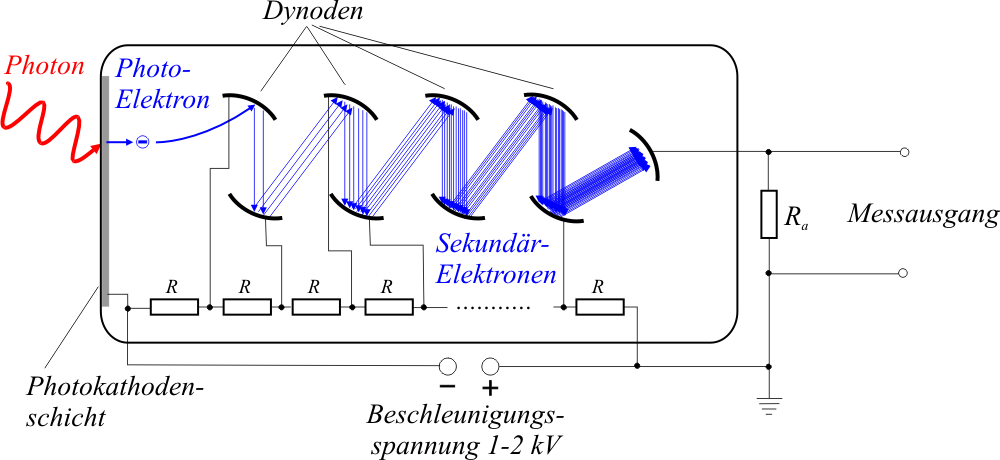
\includegraphics{../media/B3.4/Photomultiplier_schema_de.png}
	\caption{Photomultiplier (schematisch) \cite{abb:Photomultiplier}}
	\label{abb:Photomultiplier}
\end{figure}

\noindent
Um aus dem Szintillationslicht ein Messsignal zu erhalten, schließt man dem Szintillator einen Photomultiplier an. Dieser besteht aus einer Photokathode und einem Sekundärelektronenvervielfacher. Dabei muss das Emissionspektrum des Detektors optimal auf die spektrale Empfindlichkeit der Photokathode abgestimmt sein.

Die Kathode besteht entweder aus Alkali--Metallen oder Erdalkali--Metallen, die über eine geringe Elektronenaustrittarbeit verfügen.

Der zweite Bauteil heißt Sekundärelektronenvervielfacher\footnote{\emph{photomultiplier tube} (PMT)} (SEV). Dieser besitzt eine Folge von Elektroden, genannt Dynoden, die bis zu $10^7$ Sekundärelektronen pro Primärelektron erzeugen können. Zwischen den einzelnen Dynoden wird ein elektrisches Potenzial angelegt, sodass die Elektronen bis zur Anode hin beschleunigt werden. Üblicherweise haben SEVs ca. $10$ Dynoden, mit jedem Auftreffen auf eine davon werden Sekundärelektronen heraus geschlagen und vervielfacht.

Die ganze Elektronik befindet sich in einem vakuumdichten Glaskolben, der zusätzlich mit einem $\mu$--Metall--Zylinder gegen magnetische Streufelder abgeschirmt ist \cite{LMU}. Abbildung \ref{abb:Photomultiplier} zeigt den Aufbau von einem typischen Photomultiplier.

Das messbare Signal an der Anode ist dann durch richtige Kalibrierung proportional zu der im Szintillationskristall deponierten Energie des Photons aus dem $e^+ e^-$--Annihilationprozess.

\clearpage
\hypertarget{durchfuxfchrung}{%
\section{Durchführung}\label{durchfuxfchrung}}

\subsection{Einzelmessungen}
Als erstes sollen die Signale der verwendeten Elektronik einzeln am Oszilloskop betrachtet werden. Die Quelle wird für diesen Teil mittig zwischen den Detektoren platziert.

\subsubsection{Vorverstärkersignal}
In den Szintillatoren sind bereits Vorverstärker eingebaut. Der Ausgangskanal von einem der zwei Detektoren wird an ein Oszilloskops angeschlossen. Dort werden die Größe, die Lage und das Triggerlevel des Signals verändert, bis ein repräsentatives Signal gut zu erkennen ist. Dieses Signal wird gespeichert.

\subsubsection{Hauptverstärkersignal}
Daraufhin wird der Detektor mit dem Eingang des TFA angeschlossen, dessen Ausgang schließt man dann wieder an das Oszilloskop. Auch hier wird das Signal wie oben angepasst und gespeichert.

\subsubsection{Diskriminatorsignal}
Hier wird der Ausgang des TFA mit dem jeweiligen Eingang am CFD verbunden. Dessen Signale werden am Oszilloskop angeschlossen. Das Oszilloskop wird so eingestellt, dass immer dann ein Signal angezeigt wird, wenn ein logisches Signal detektiert wird.

\subsubsection{Einstellung der Diskriminatoren}
Mit dem CFD können jetzt Signale verschiedener Energie entweder zugelassen oder herausgefiltert werden. Dazu werden die Schwellen von oben und unten manuell eingestellt, bis am Oszilloskop bestimmte Signale nicht mehr zu sehen sind.

Für die nächsten zwei Versuchsteile werden die CFD so eingestelllt, sodass nur Photonen mit $\pu{511\, keV}$ dargestellt werden. Anschließend werden die Diskriminatoren an die Koinzidenzeinheit angeschlossen.

\subsection{Ortsauflösung}
\label{sec:Ortsauflösung}
In diesem Teil soll der Einfluss der Lage der Quelle bezüglich der Verbindungsline der Szintillatoren auf die Koinzidenzzählrate untersucht werden.

Dafür wird die Quelle mittig auf den Wagen platziert. Dann verschiebt man den Wagen durch den Bereich, der vom Detektor abgedeckt wird und misst die Zählrate für jeweils $60\,\mathrm{s}$. Erwartet wird eine gaußförmige Verteilung der Zählraten, deshalb sollte im Bereich der Halbwertbreiten und Hochpunkt kleinere Abstände gewählt werden. Es werden mindesten $20$ Messungen in einem Raumintervall von $\pm 50\,\mathrm{mm}$ durchgeführt.

In den Abständen von $\pm 8\,\mathrm{mm}$ wurden minimale Abstände von $\pm 1\,\mathrm{mm}$ zwischen den Positionen verändert, weiter außen wurden größere Abstände gewählt. Die Ungenauigkeit beim Einstellen der Position wird auf $\pu{\pm 2\, mm}$ gesetzt.

\subsection{PET--Scan der Truhe}
Vom Betreuer wurde eine verschlossene Truhe vorbereitet, in der sich mehrere Quellen verschiedener Intensität befinden konnten.  Ziel dieses Versuchsteils ist die Ortung von verschiedenen Proben in unbekannter Anordnung.

Die Truhe besitzt $100$ mögliche Steckplätzen in einem $10\times10$--Raster. Um dieses zu beschreiben, werden die Richtungen $x$, $y$ und $z$ definiert und in Abbildung \ref{abb:TruheRichtungen} dargestellt. Es gibt je $10$ Reihen in $x$-- und $y$--Richtung sowie $19$ Reihen in $z$--Richtung.

Die Abstände zwischen zwei $x$-- bzw. $y$--Reihen betragen $\pu{1\,cm}$, die Abstände zwischen zwei $z$--Reihen betragen $(\sqrt{2})^{-1}\,\mathrm{cm}$. Alle Messungen erfolgen über eine Dauer von $60\,\mathrm{s}$.

\begin{figure}[h]
	\centering
	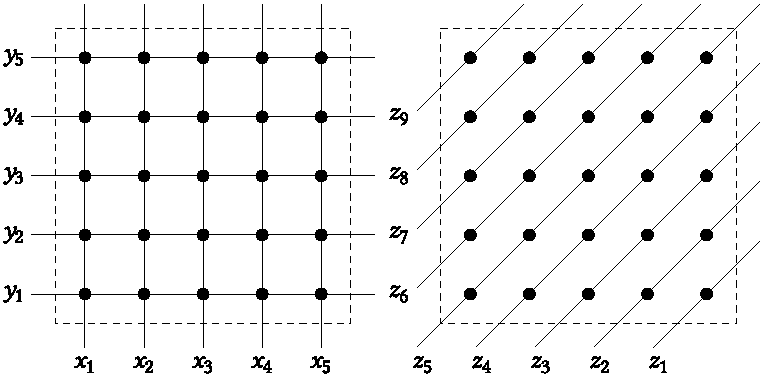
\includegraphics{../media/B3.4/Box_Axis.pdf}
	\caption{Richtungsdefinitionen (schematisch) \cite{UzK}}
	\label{abb:TruheRichtungen}
\end{figure}

An den Positionen $(7,8)$ und $(10,4)$ sind ziemlich sicher Proben zu erwarten. Weiterhin soll eine Probe bei $(3, 2)$ positioniert sein, dies allerdings für uns nicht aus den Werten ersichtlich.

\subsection{Winkelabhängigkeit}
In diesem Teil soll die Kollinearität der Photonen aus der $e^+e^-$-Paarvernichtung nachgewiesen werden.

Wie bei der Messung der \nameref{sec:Ortsauflösung} wird eine Probe offen und mittig positioniert.

Einer der Detektoren wird in einem Winkel zwischen $\pm 5\,^\circ$ zur Verbindungslinie eingestellt. Die Winkelveränderungen werden in Schritten von $0,5\,^\circ$ eingestellt, wiederum dauert jede Messung $60\,\mathrm{s}$. Der Fehler des Winkels wird auf $\Delta \theta = \pu{0,5\,^\circ}$ geschätzt.

Zunächst werden beide Detektoren wie in den letzten Versuchsteilen auf Energien von $\pu{511\,keV}$ eingestellt. Ebenso wie bei der Ortsauflösung wird eine Gaußverteilung der Zählraten erwartet.

Daraufhin wird einer der Detektoren auf eine Energie von $\pu{1275\,keV}$ eingestellt. Dies entspricht der Energie des sekundären $\gamma$--Zerfalls von $\ce{^{22}Ne}$ in den Grundzustand, der koinzident mit dem $\beta^+$--Zerfall stattfindet. Da dieser zweite Zerfall in alle Raumrichtungen erfolgt, wird eine näherungsweise konstante, kleine Zählrate erwartet.

\clearpage
\hypertarget{auswertung}{%
\section{Auswertung}\label{auswertung}}

\subsection{Signale am Oszilloskop}
Das initiale Messsignal, das von den Detektoren erzeugt wird, unterliegt mehreren Veränderungen durch die anderen elektronischen Bauteile, bevor es den Zähler erreicht. Die unterschiedlichen Stufen dieser Veränderung werden im Folgenden genauer untersucht

\subsubsection{Signal aus dem Vorverstärker}
Das Signal aus dem Vorverstärker ist in Abbildung \ref{fig:signal_vv} zu sehen. Es hat eine Breite von ca. $150 \mathrm{\, \mu s}$ und am Peak eine Höhe von ca. $400 \mathrm{\, mV}$. Damit ist das Signal noch recht breit und besitzt daher noch keine herausragende zeitliche Auflösung.

\begin{figure}[h]
	\centering
	\includegraphics[width=0.7\textwidth]{../media/B3.4/Signal_Vorverstärker.jpg}
	\caption{Signal aus dem Vorverstärker}
	\label{fig:signal_vv}
\end{figure}

\subsubsection{Signal aus dem Hauptverstärker}
Das Signal aus dem TFA ist in Abbildung \ref{fig:signal_vv+hv} zu sehen. Es hat eine Breite von ca. $850 \mathrm{\, ns}$ und beim Peak eine Höhe von ca. $2,5 \mathrm{\, V}$. Damit ist es etwa $175$--mal schmaler und $6$--mal höher als das Signal aus dem Vorverstärker. Der TFA hat das Signal daher sowohl stark verstärkt, als auch die zeitliche Auflösung enorm vergrößert.

\begin{figure}[h]
	\centering
	\includegraphics[width=0.7\textwidth]{../media/B3.4/Signal_Hauptverstärker.jpg}
	\caption{Signal aus dem Hauptverstärker}
	\label{fig:signal_vv+hv}
\end{figure}

\subsubsection{Signal aus dem CFD}
Die finale Veränderung des Signals ist in Abbildung \ref{fig:signal_cfd} zu sehen. In gelb ist das Signal abgebildet, das der CFD konstruiert, wie es in Abschnitt \ref{cfd} beschrieben ist. Dabei ist zu beachten, dass der Teil der Kurve, der unterhalb der x-Achse verläuft, in Abbildung \ref{fig:signal_cfd} nicht zu sehen ist. Dieser wurde nur selten angezeigt und konnte somit nicht gut aufgenommen werden.

\begin{figure}[h]
	\centering
	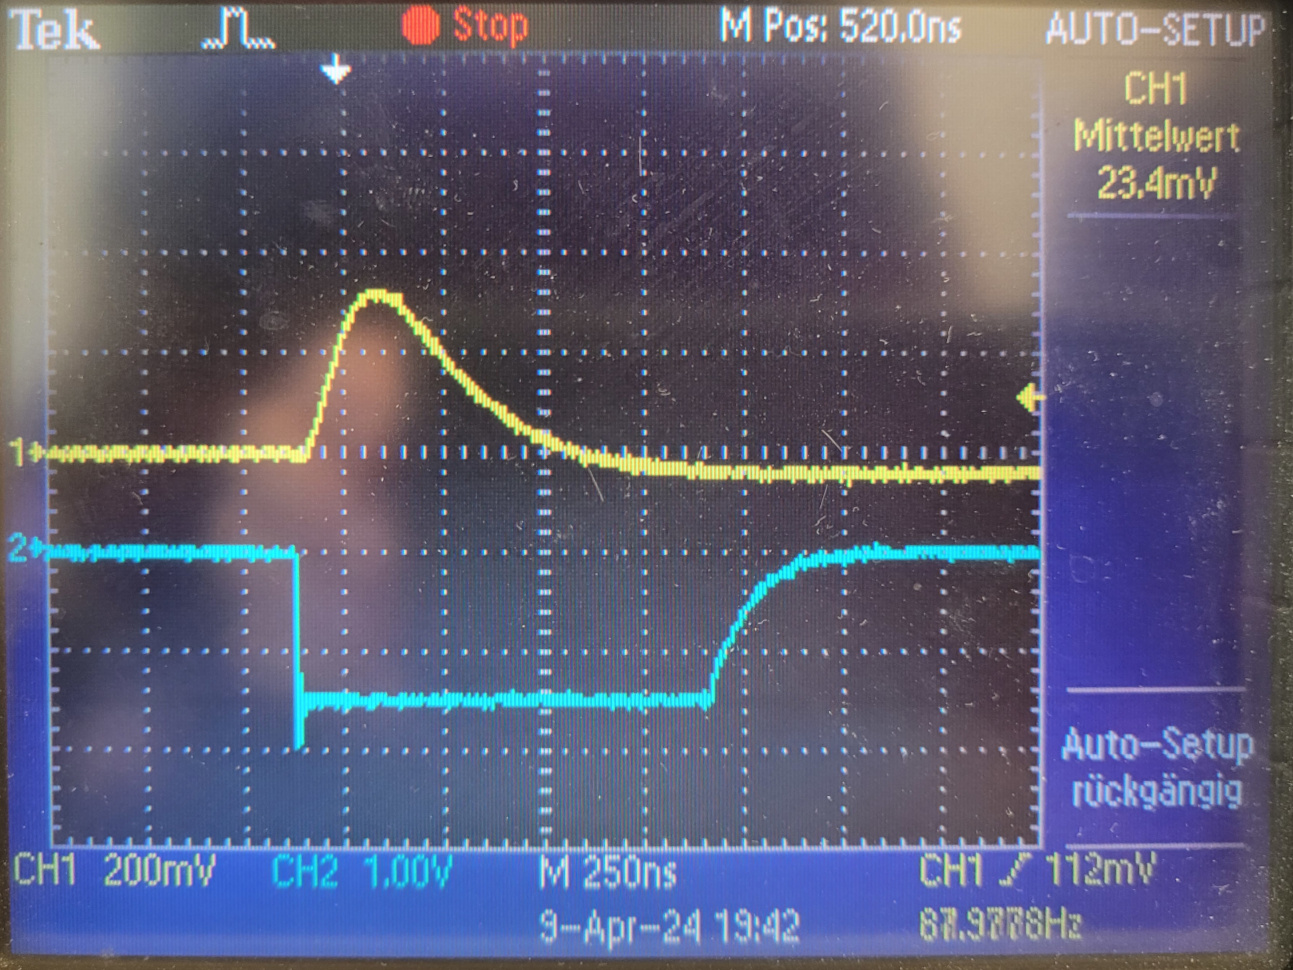
\includegraphics[width=0.7\textwidth]{../media/B3.4/Signal_CFD.jpg}
	\caption{Vom CFD kombiniertes eintreffendes Signal (gelb) und logisches Signal (blau)}
	\label{fig:signal_cfd}
\end{figure}

Es hat eine Breite von ca. $625 \mathrm{\, ns}$ und beim Peak eine Höhe von ca. $300 \mathrm{\, mV}$. Damit ist das Signal ungefähr so breit wie das aus dem TFA, die zeitliche Auflösung wurde durch das CFD  daher kaum verändert. Die Höhe ist wieder deutlich kleiner, aber die Information der Höhe ist für die Ausgabe des CFDs nicht von Relevanz und kann damit hier ohne Probleme wieder verringert werden.

In blau ist das vom CFD ausgegebene logische Signal zu sehen. Es hat die Charakteristik eines klassischen Kastensignals, ist ca. $1,25 \mathrm{\, \mu s}$ breit und ca. $300 \mathrm{\, mV}$ hoch. Die Höhe und Breite sind beide fest eingestellt und unabhängig vom eintreffenden Signal, weshalb hier kein direkter Vergleich angebracht ist. Bemerkenswert ist trotzdem, dass die Breite des logischen Signals sehr ähnlich zur Breite des eintreffenden Signals ist. Daran ist zu sehen, dass die Breite des logischen Signals sinnvoll eingestellt ist, da sie die zeitliche Auflösung weder stark verringert noch erhöht.

\hypertarget{auswertung-ortsaufluxf6sung}{\subsection{Ortsauflösung}\label{auswertung-ortsaufluxf6sung}}
Zur Bestimmung der Ortsauflösung wird die Zählrate $r$ aus der Anzahl der Detektionen $n$ und der Messdauer $T_\mathrm{Ort}=60\,\mathrm{s}$ bestimmt. Der Fehler der Detektionszahl $\Delta n$ folgt aus statistischer Streuung, der Fehler der Zählrate $\Delta r$ folgt nach Gauß'scher Fehlerfortpflanzung. Hierbei kann die Messdauer als näherungsweise exakt angenommen werden, der Messfehler in der Zeit ist vernachlässigbar. Die Ergebnisse sind in Tabelle \ref{tab:Ortsauflösung} dargestellt.

\begin{eqnarray}
	\Delta n &=& \sqrt{n} \label{eq:Delta n} \\
	r &=& \frac{n}{T_\mathrm{Ort}} \label{eq:Zählrate} \\
	\Delta r &=& \frac{\Delta n}{T_\mathrm{Ort}} \label{eq:ZählrateFehler}
\end{eqnarray}


\begin{table}[h]
	\centering
	\begin{tabular}{c|c|c||c|c|c}
		$x\ [\mathrm{mm}]$ & $n\ [\frac{1}{\mathrm{min}}]$ & $r\ [\mathrm{Hz}]$ &
		$x\ [\mathrm{mm}]$ & $n\ [\frac{1}{\mathrm{min}}]$ & $r\ [\mathrm{Hz}]$ \vspace{1pt}\\
		\hline
		$\ \ \ 0 \pm 2$ & $2971 \pm 55$ & $49,52 \pm 0,91$ &---&---&--- \\
		$\ +1 \pm 2$ & $2202 \pm 47$ & $36,70 \pm 0,78$ &
		$\ -1 \pm 2$ & $1650 \pm 41$ & $27,50 \pm 0,68$ \\
		$\ +2 \pm 2$ & $1616 \pm 40$ & $26,93 \pm 0,67$ &
		$\ -2 \pm 2$ & $\ 938 \pm 31$ & $15,63 \pm 0,51$ \\
		$\ +3 \pm 2$ & $\ 686 \pm 26$ & $11,43 \pm 0,44$ &
		$\ -3 \pm 2$ & $\ 493 \pm 22$ & $\ 8,22 \pm 0,37$ \\
		$\ +4 \pm 2$ & $\ 512 \pm 23$ & $\ 8,53 \pm 0,38$ &
		$\ -4 \pm 2$ & $\ 477 \pm 22$ & $\ 7,95 \pm 0,36$ \\
		$\ +5 \pm 2$ & $\ 538 \pm 23$ & $\ 8,97 \pm 0,39$ &
		$\ -5 \pm 2$ & $\ 486 \pm 22$ & $\ 8,10 \pm 0,37$ \\
		$\ +6 \pm 2$ & $\ 498 \pm 22$ & $\ 8,30 \pm 0,37$ &
		$\ -6 \pm 2$ & $\ 511 \pm 23$ & $\ 8,52 \pm 0,38$ \\
		$\ +7 \pm 2$ & $\ 467 \pm 22$ & $\ 7,78 \pm 0,36$ &
		$\ -7 \pm 2$ & $\ 414 \pm 20$ & $\ 6,90 \pm 0,34$ \\
		$\ +8 \pm 2$ & $\ 487 \pm 22$ & $\ 8,12 \pm 0,37$ &
		$\ -8 \pm 2$ & $\ 405 \pm 20$ & $\ 6,75 \pm 0,34$ \\
		$+11 \pm 2$ & $\ 335 \pm 18$ & $\ 5,58 \pm 0,31$ &---&---&---\\
		$+15 \pm 2$ & $\ 249 \pm 16$ & $\ 4,15 \pm 0,26$ &
		$-15 \pm 2$ & $\ 229 \pm 15$ & $\ 3,82 \pm 0,25$ \\
		$+20 \pm 2$ & $\ 170 \pm 13$ & $\ 2,83 \pm 0,22$ &
		$-20 \pm 2$ & $\ 159 \pm 13$ & $\ 2,65 \pm 0,21$ \\
		$+30 \pm 2$ & $\ \ 95 \pm 10$ & $\ 1,58 \pm 0,16$ &
		$-30 \pm 2$ & $\ 112 \pm 11$ & $\ 1,87 \pm 0,18$ \\
		$+50 \pm 2$ & $\ 78 \pm 9$ & $\ 1,30 \pm 0,15$ &---&---&---
	\end{tabular}
	\caption{Messergebnisse der Ortsauflösung}
	\label{tab:Ortsauflösung}
\end{table}

\noindent
Diese Daten sind in Abbildung \ref{abb:zaehlrate} dargestellt und gefittet worden. Dabei wurde eine Gaußverteilung angenommen. Dabei wurden der Mittelwert $\mu\approx 0,33\,\mathrm{mm}$, eine Standardabweichung $\sigma\approx1,37\,\mathrm{mm}$, ein Streckungsfaktor $\alpha\approx 40\,\mathrm{Hz}$ und ein Offset von $\beta\approx 5,69\,\mathrm{Hz}$ ermittelt.

\begin{eqnarray}
    \phi(x, \mu, \sigma, \alpha, \beta) &=& \alpha\cdot \exp\left[- \frac{(x - \mu)^2}{2\sigma^2} \right] + \beta \label{eq:gauss-fit}
\end{eqnarray}

\noindent
Die Ortsauflösung kann durch die ermittelte Standardabweichung bestimmt werden. Allerdings sieht man, dass auch außerhalb des Peaks erhöhte Werte gemessen werden. Daher wird die Messgenauigkeit durch die Auflösung auf $\Delta x_\mathrm{res}=\pm 1,9\,\mathrm{mm}$ festgelegt. Da schon bei der Messung ein Fehler $\Delta x=\pm 2\,\mathrm{mm}$ verwendet wurde, nimmt die Ungenauigkeit durch die Auflösung einen geringeren Einfluss auf die Messgenauigkeit und kann vernachlässigt werden.

\begin{figure}[h]
	\centering
	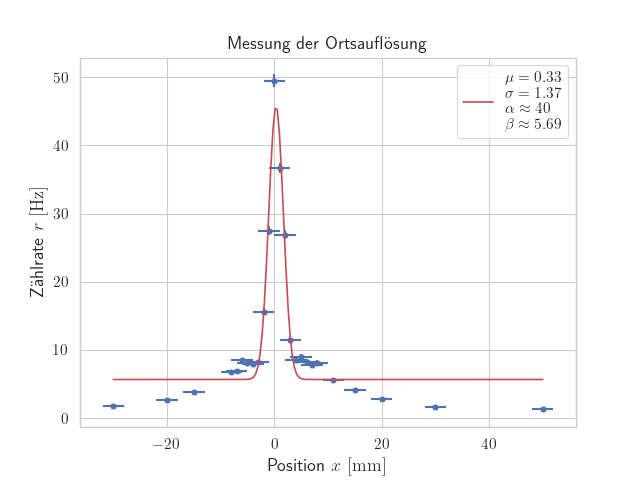
\includegraphics[width=0.9\textwidth]{../media/B3.4/Ortsaufloesung_fit.png}
	\caption{Zählraten}
	\label{abb:zaehlrate}
\end{figure}

\clearpage
\hypertarget{petscan}{%
\subsection{PET--Scan}\label{petscan}}
In $x$-- und $y$--Richtung wurden je $10$ Messungen durchgeführt. Die Fehler der Zählraten $N$ sind dabei durch die statistische Streuung \eqref{eq:Delta n} bestimmt. Die Ergebnisse sind in Tabelle \ref{tab:PET x y} dargestellt.

Anhand der Werte kann man schon erahnen, dass es mindesten vier Positionen gibt, an denen sich Proben befinden könnten. Um die richtigen Positionen herauszufiltern, müssen die Messungen in $z$--Richtung betrachtet werden. Diese sind in Tabelle \ref{tab:PET z} dargestellt.

Aus diesen Werten lässt sich schließen, dass mindestens zwei starke Quellen positioniert wurden. Um genauer sagen zu können, werden die Zählraten zu einer Position $(x,y,z)$ miteinander multipliziert und als Heatmap sowie als Oberflächenplot visualisiert, siehe Abbildungen \ref{abb:PET heatmap} und \ref{abb:PET surface} sowie Tabelle \ref{tab:PET Matrix}. Es ist deutlich zu sehen, dass zwei große Quellen an den Positionen $(10,4)$ und $(7,9)$ positioniert sind.

Ein Foto der verschlossenen Box und eine Überlagerung mit der Heatmap sind in den Abbildungen \ref{abb:PET box} und \ref{abb:heatmap & Box} zu sehen.

\begin{figure}[b!]
	\centering
	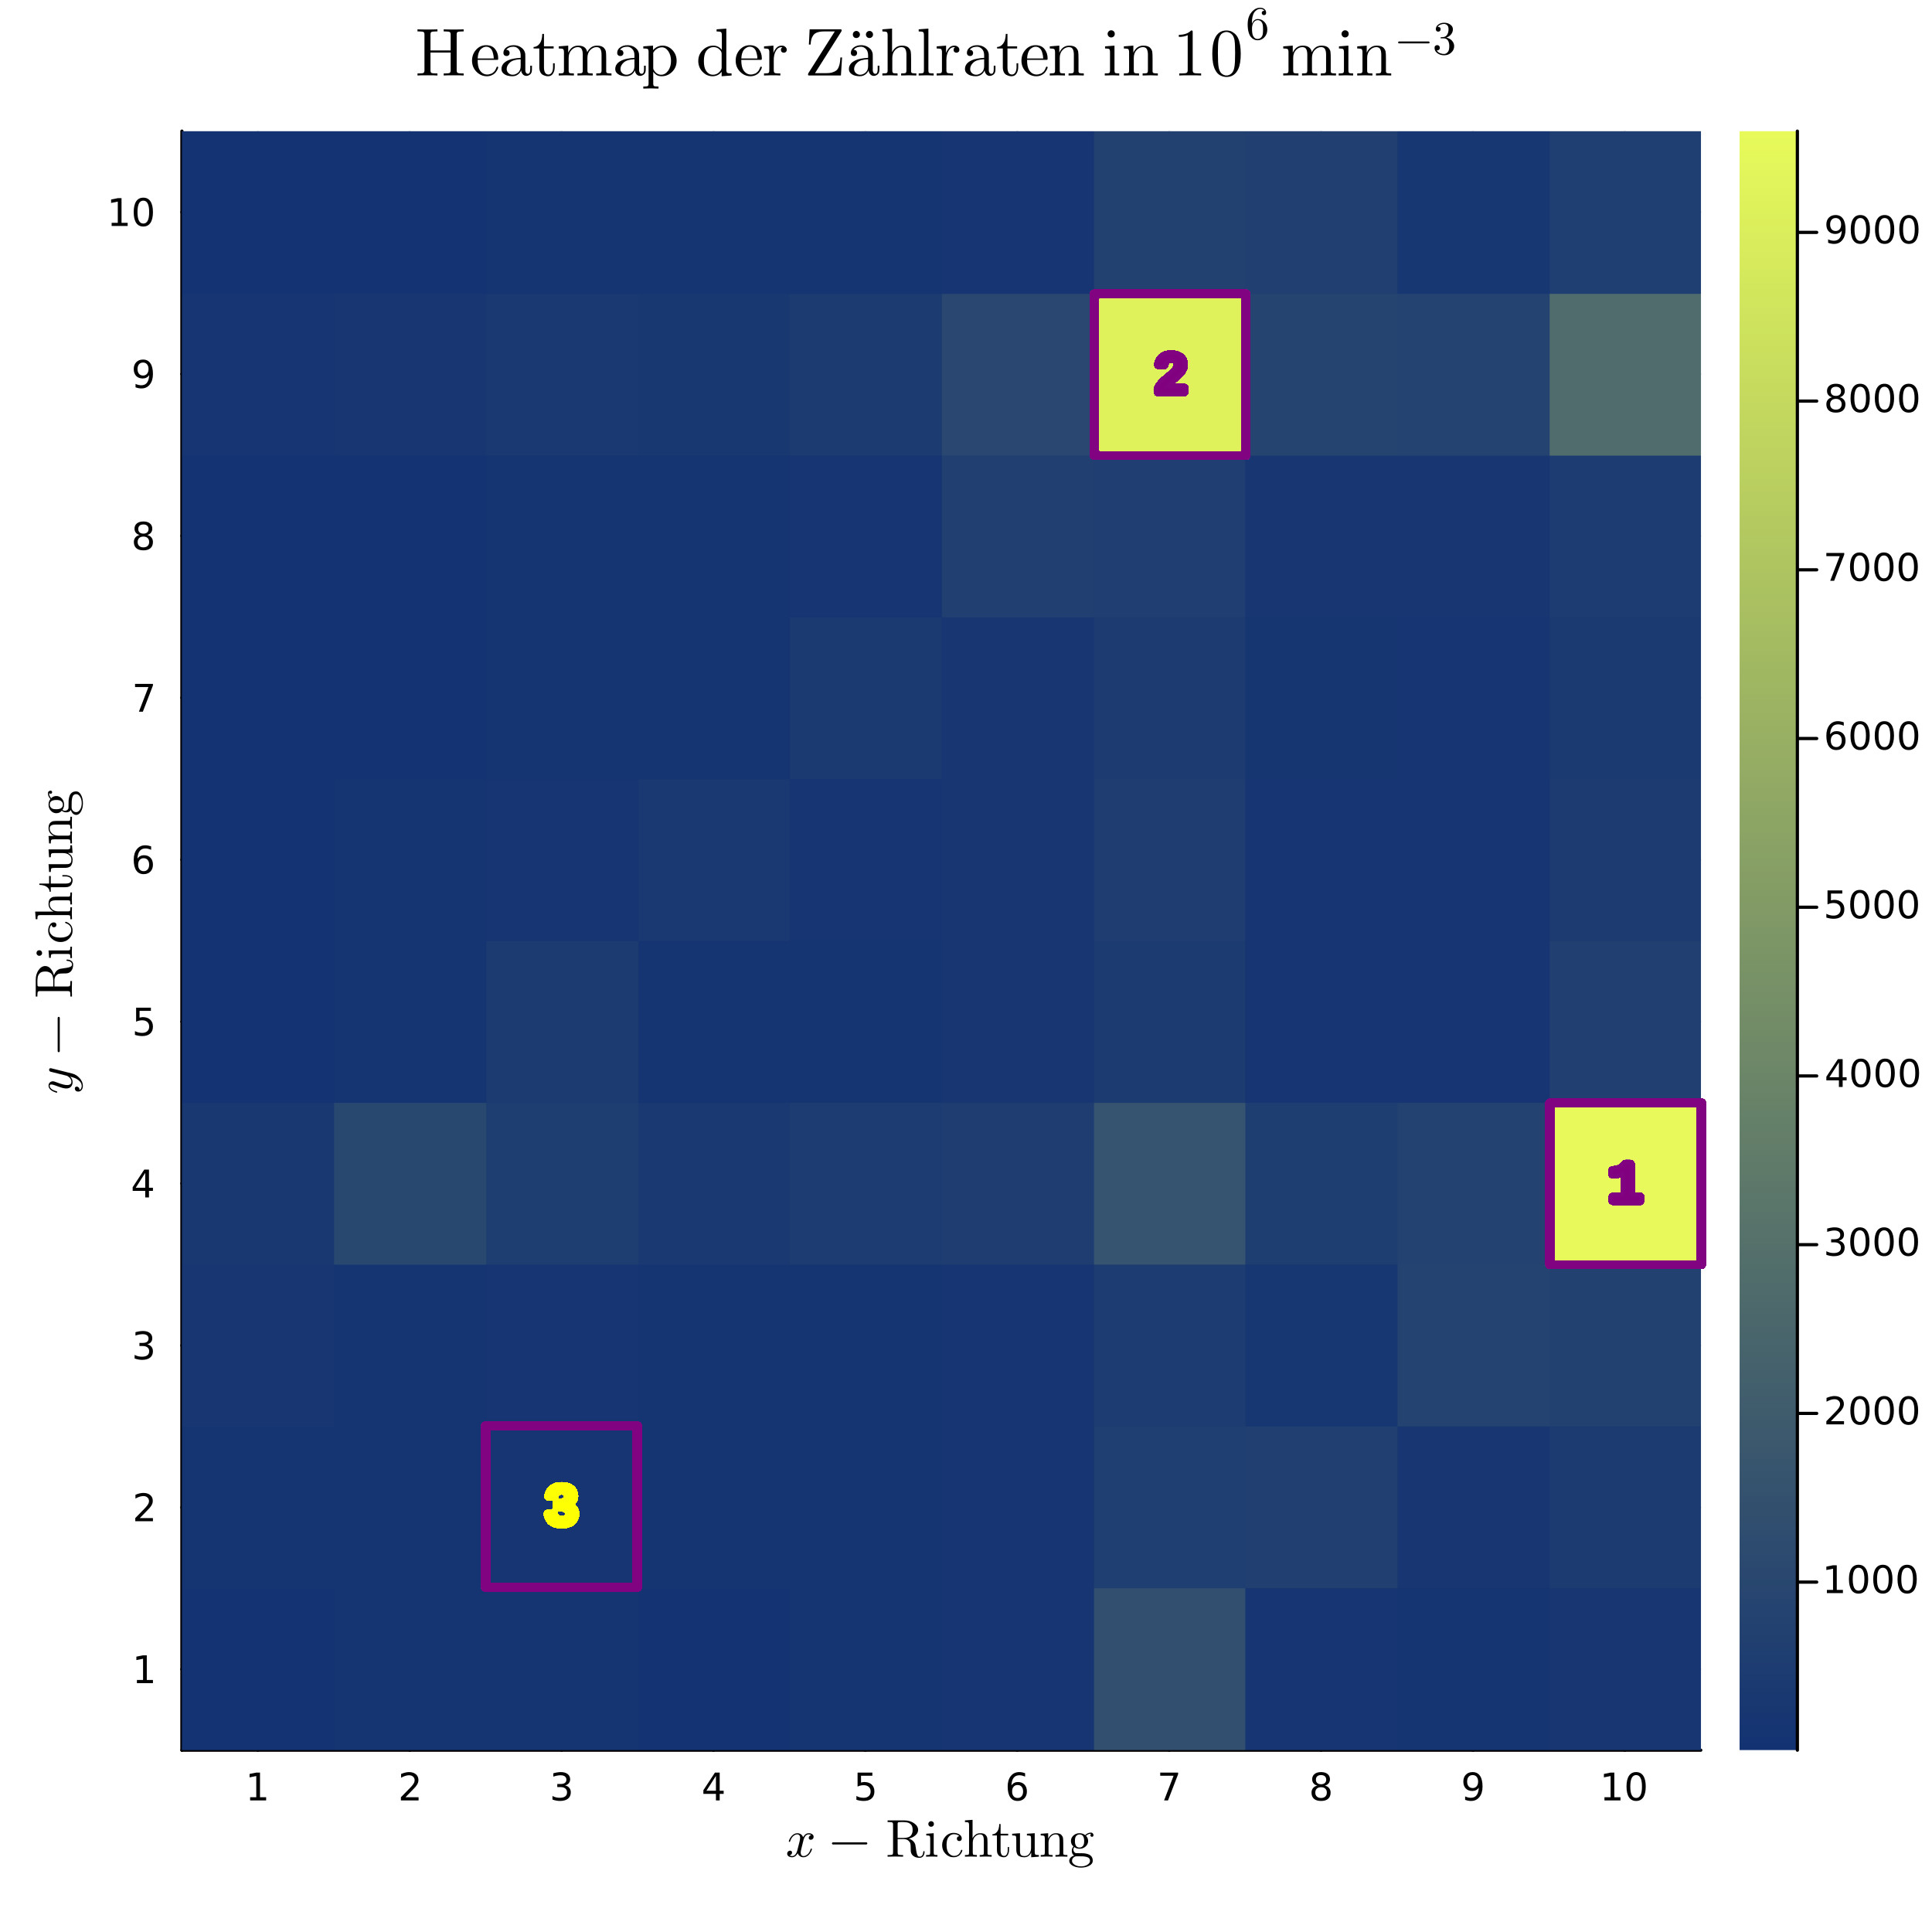
\includegraphics[width=0.7\textwidth]{../media/B3.4/heatmap.jpg}
	\caption{Heatmap, $z$--Richtung läuft diagonal von oben links nach unten rechts}
	\label{abb:PET heatmap}
\end{figure}

\begin{figure}[h!]
	\centering
	\begin{minipage}{0.43\textwidth}
		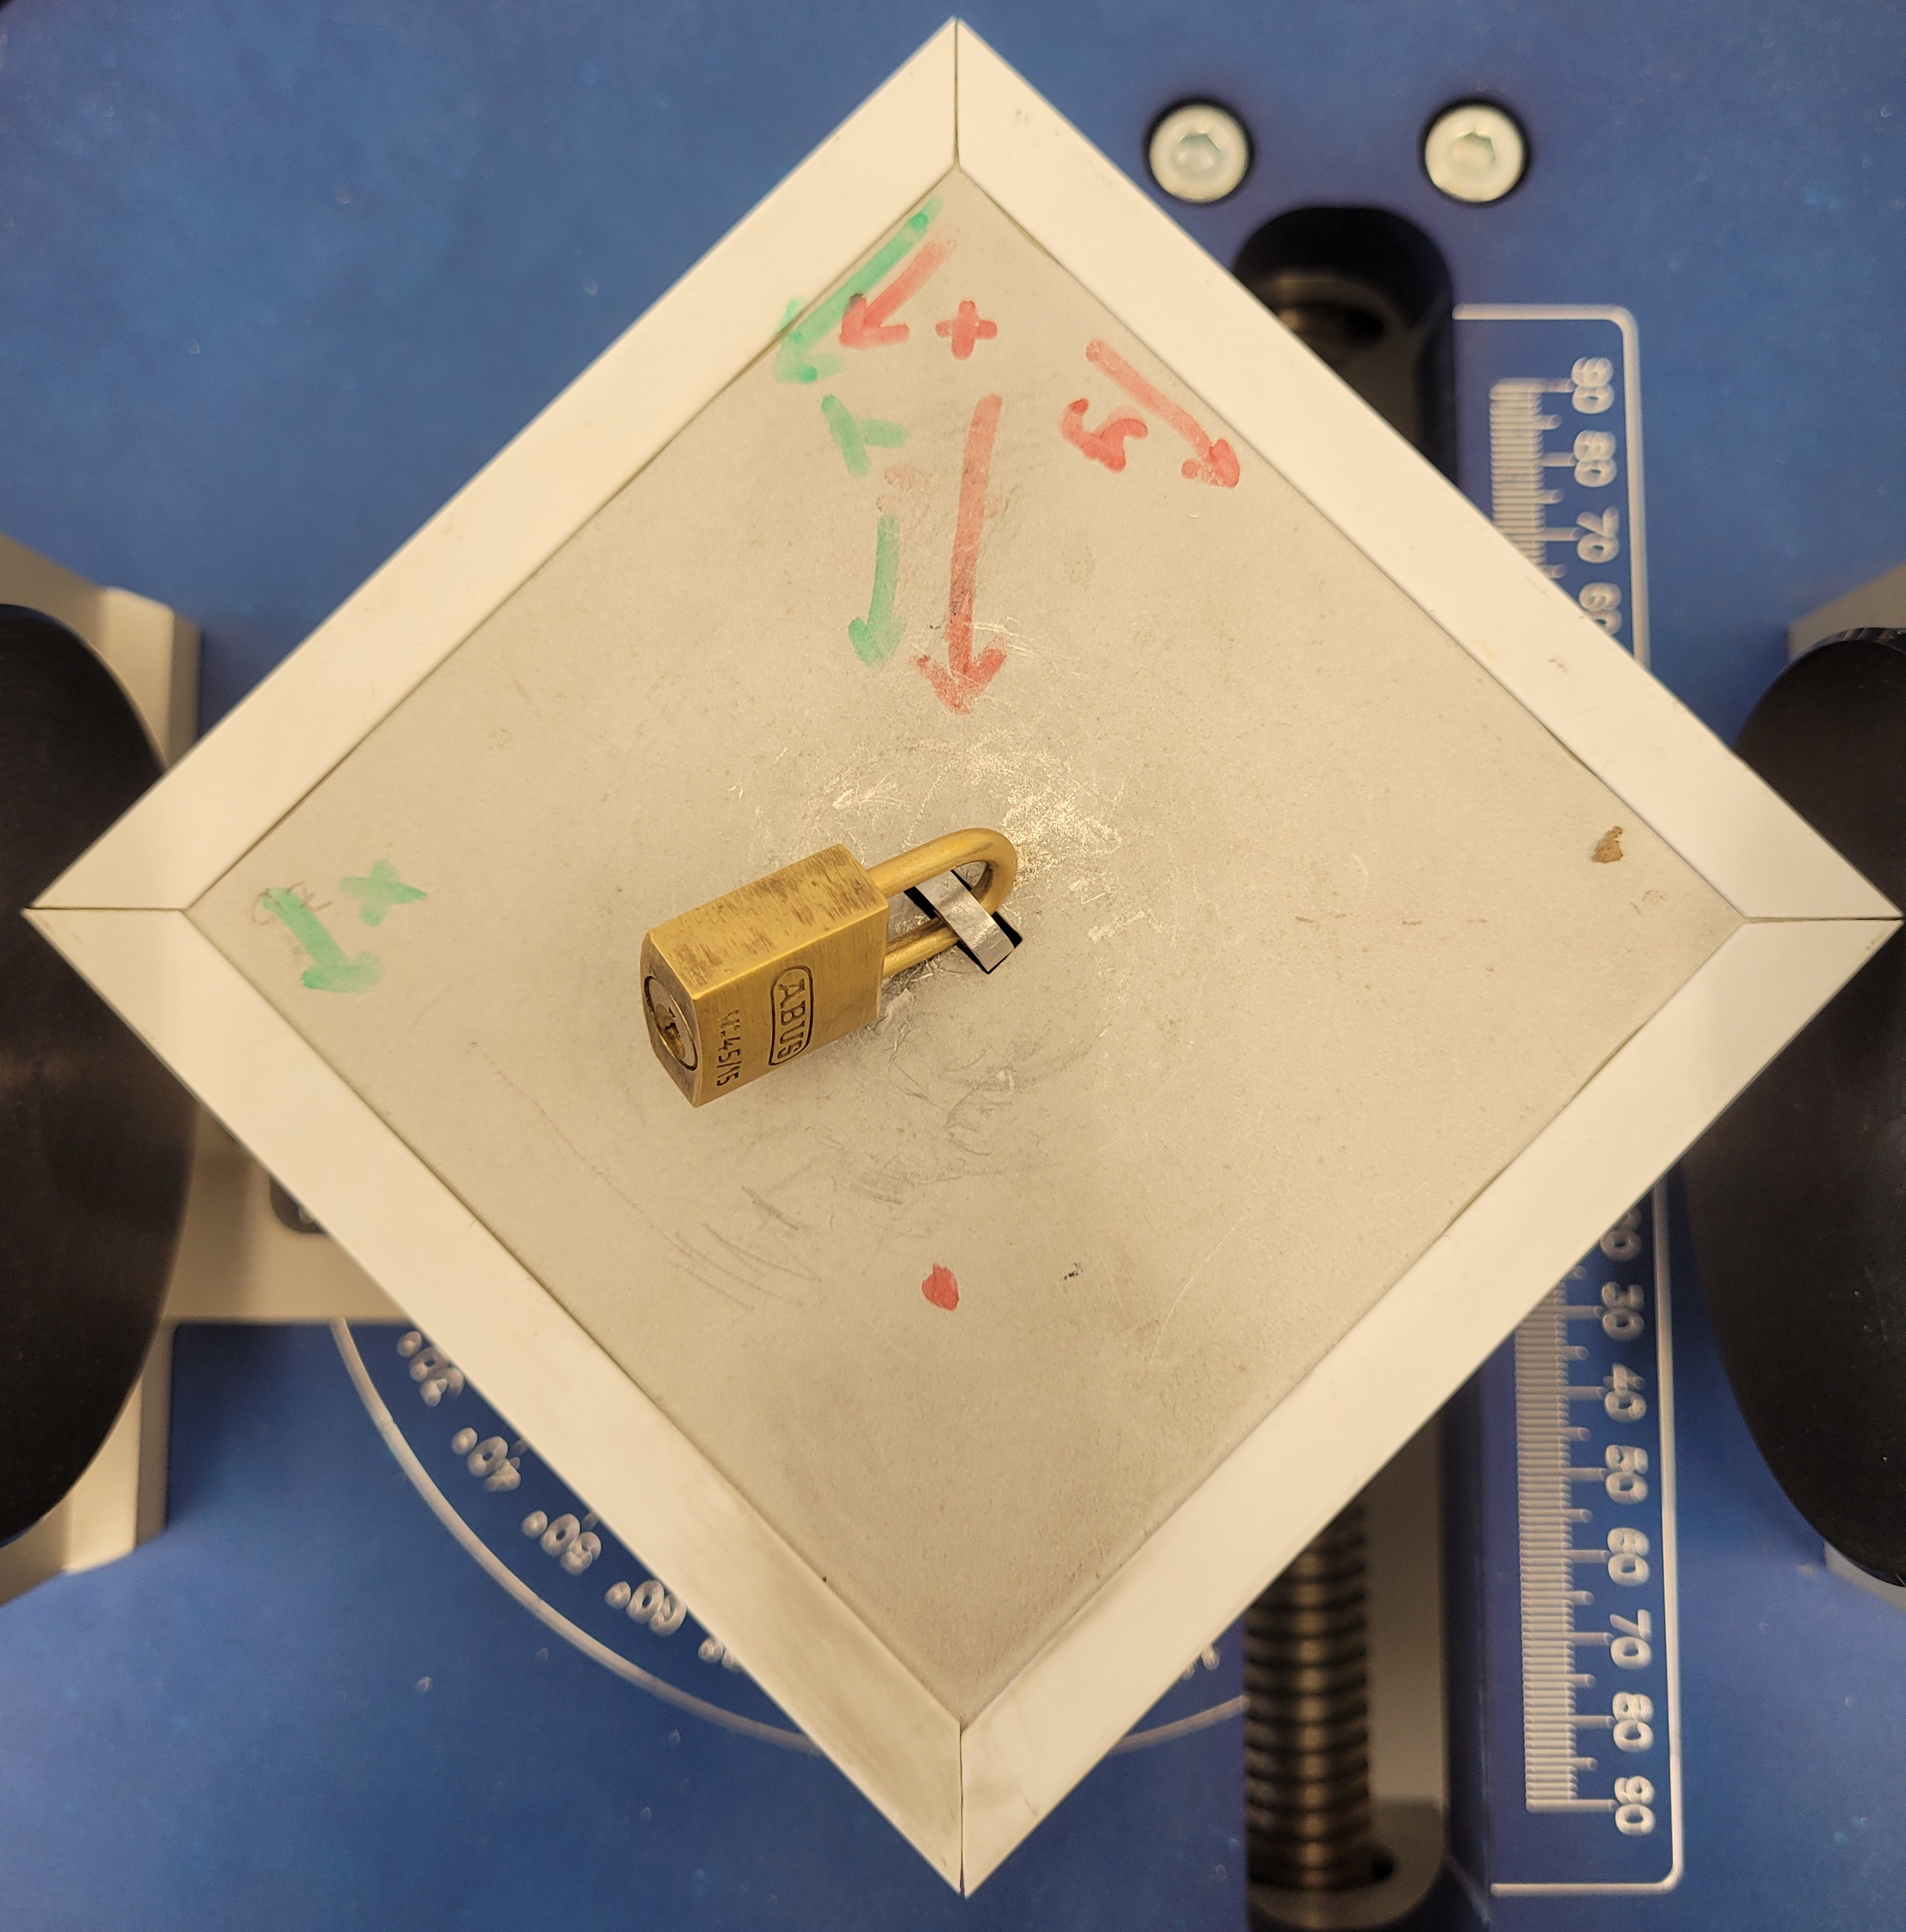
\includegraphics[width=\textwidth]{../media/B3.4/Box_von_oben.jpg}
		\caption{Verschlossene Box zur PET--Messung}
		\label{abb:PET box}
	\end{minipage}
	\begin{minipage}{0.45\textwidth}
		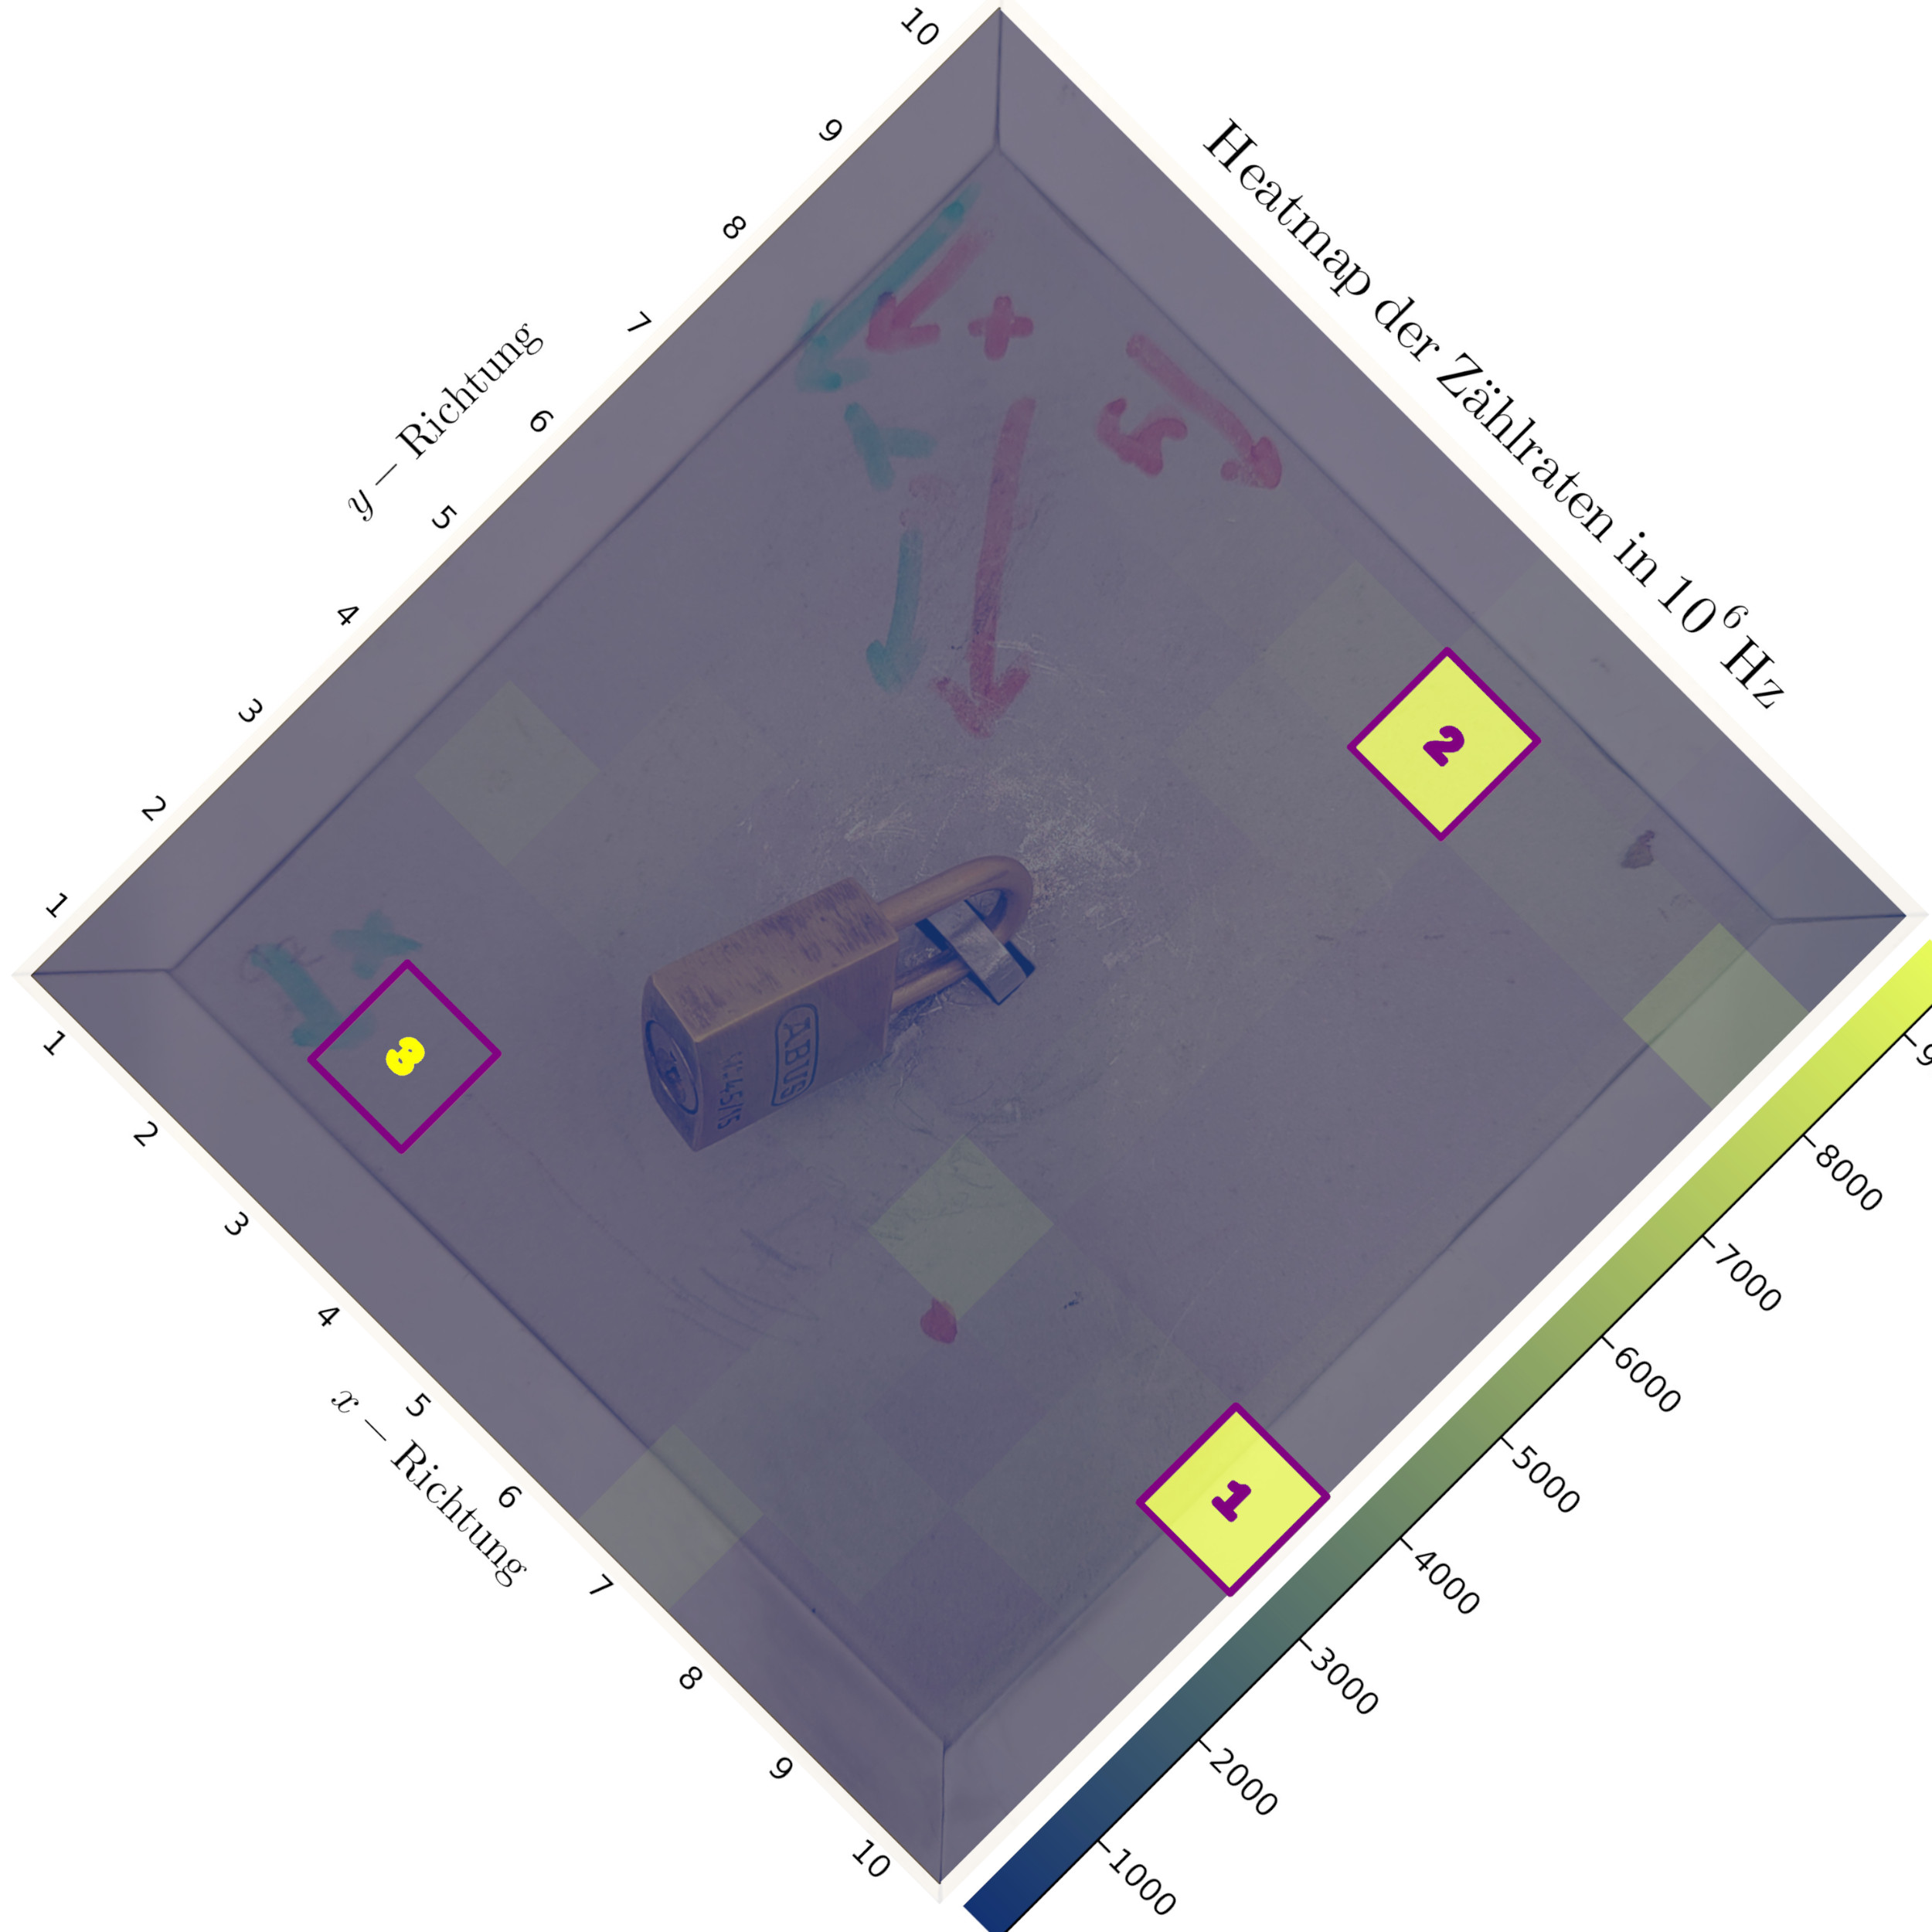
\includegraphics[width=\textwidth]{../media/B3.4/heatmap_with_box.jpg}
		\caption{Überlagerung der Heatmap mit der Box}
		\label{abb:heatmap & Box}
	\end{minipage}
\end{figure}

\begin{figure}[h!]
	\centering
	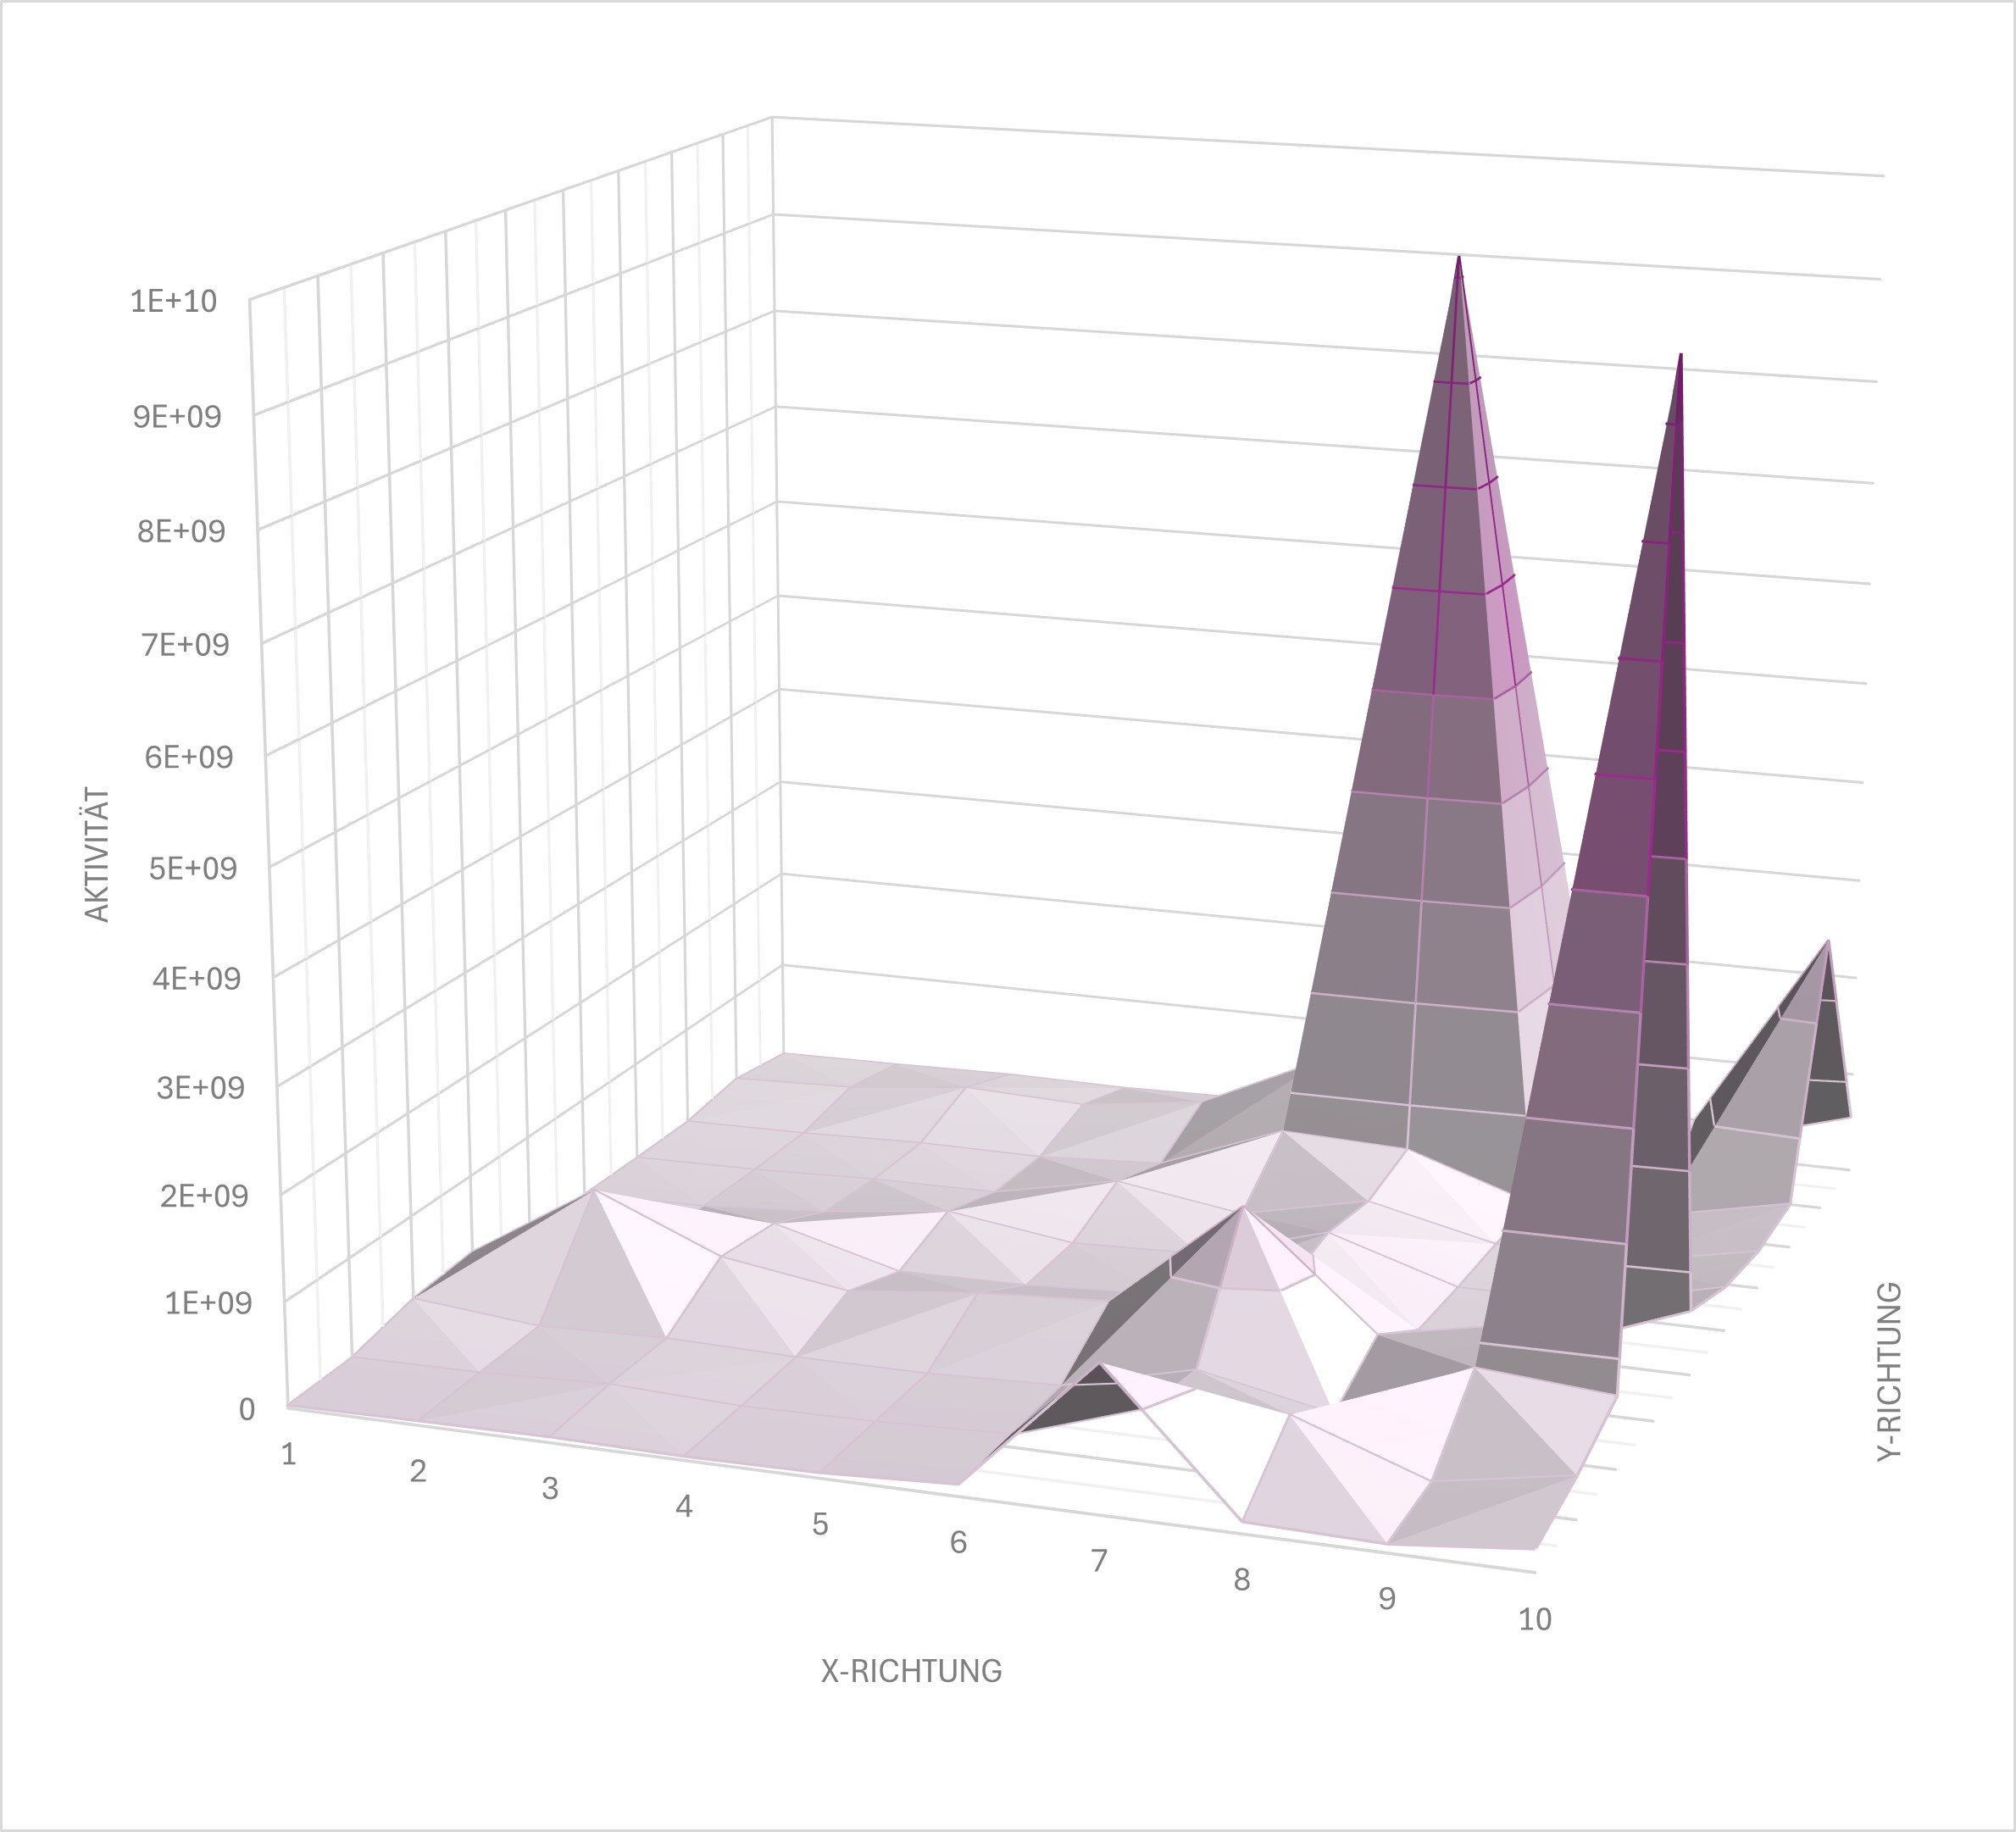
\includegraphics[width=0.8\textwidth]{../media/B3.4/PET_surface.jpg}
	\caption{Oberflächenplot in $3\,\mathrm D$}
	\label{abb:PET surface}
\end{figure}

Uns wurde mitgeteilt, es gebe eine dritte, schwächere Probe. Weder anhand der Daten noch anhand der Grafiken können wir diese Quelle lokalisieren, weil es kaum signifikante Abhebungen erkennbar sind. Vermutlich ist diese sehr viel schwächer als die zwei große Quellen.

Betrachtet man die Werte sehr genau, kann man $(3,2)$ als mögliche Position einer dritten Quelle vermuten. Der Messwert $N(z_{11})$ ist größer als die benachbarten Messungen in der $z$--Richtung. Weiterhin ist Produkt der Zählraten an Position $(3,2)$ deutlich höher als die meisten benachbarten Werte, siehe Tabelle \ref{tab:PET Matrix}.

Definiert man das Produkt aus den Zählraten der drei Richtungen als Aktivität, so ist diese Aktivität  $A_1$ von Quelle $1$ an der Position $(10,4)$ um etwa $4\,\%$ höher als die von Quelle $2$ an der Position $(7,9)$. Eine mögliche Quelle $3$ an Position $(3,2)$ ist deutlich schwächer, sie hat nur ca $1\,\%$ der Aktivität der beiden anderen Proben. Dies erklärt, warum sie im Unterschied zu den anderen beiden Quellen praktisch nicht identifizierbar ist.

\begin{eqnarray}
	\frac{A_1}{A_2} &\approx& 104\,\% \\
	\frac{A_3}{A_1} &\approx& 1,12\,\% \\
	\frac{A_3}{A_2} &\approx& 1,15\,\%
\end{eqnarray}

\begin{table}
	\centering
	\begin{tabular}[h]{c|c|r|r}
		Nr. & Position [mm] & N(x) $[\frac{1}{\mathrm{min}}]$ & N(y) $[\frac{1}{\mathrm{min}}]$ \vspace{1pt}\\
		\hline
		1 & $-45 \pm 2$ & $190 \pm 14$ & $313 \pm 18$ \\
		2 & $-35 \pm 2$ & $261 \pm 16$ & $466 \pm 22$ \\
		3 & $-25 \pm 2$ & $440 \pm 21$ & $542 \pm 23$ \\
		4 & $-15 \pm 2$ & $312 \pm 18$ & $2021 \pm 45$ \\
		5 & $-\ \ 5 \pm 2$ & $414 \pm 20$ & $498 \pm 22$ \\
		6 & $+\ \ 5 \pm 2$ & $639 \pm 25$ & $481 \pm 22$ \\
		7 & $+15 \pm 2$ & $2025 \pm 45$ & $431 \pm 21$ \\
		8 & $+25 \pm 2$ & $616 \pm 25$ & $503 \pm 22$ \\
		9 & $+35 \pm 2$ & $660 \pm 26$ & $2385 \pm 49$ \\
		10 & $+45 \pm 2$ & $2186 \pm 47$ & $520 \pm 23$
	\end{tabular}
	\caption{Messwerte des PET--Scans in $x$-- und $y$--Richtung}
	\label{tab:PET x y}
	
	\vspace{24pt}
	\begin{tabular}{c|c|r||c|c|r}
		Index $i$ &
			Position $[\mathrm{mm}]$ &
			$N(z_i)$ $[\frac{1}{\mathrm{min}}]$&
			Index $i$ &
			Position $[\mathrm{mm}]$ &
			$N(z_i)$ $[\frac{1}{\mathrm{min}}]$ \vspace{1pt}\\
		\hline
		$1$ & $64 \pm 2$ & $203 \pm 14$&
		$11$ & $-\ 7 \pm 2$ & $524 \pm 23$ \\
		$2$ & $57 \pm 2$ & $246\pm 16$&
		$12$ & $-14 \pm 2$ & $397 \pm 20$ \\
		$3$ & $49 \pm 2$ & $243\pm 16$ &
		$13$ & $-21 \pm 2$ & $384 \pm 20$ \\
		$4$ & $42 \pm 2$ & $271 \pm 16$ &
		$14$ & $-28 \pm 2$ & $401 \pm 20$ \\
		$5$ & $35 \pm 2$ & $318 \pm 18$ &
		$15$ & $-35 \pm 2$ & $562 \pm 24$ \\
		$6$ & $28 \pm 2$ & $407 \pm 20$ &
		$16$ & $-42 \pm 2$ & $2173 \pm 47$ \\
		$7$ & $21 \pm 2$ & $644 \pm 25$ &
		$17$ & $-49 \pm 2$ & $571 \pm 24$ \\
		$8$ & $14 \pm 2$ & $1907 \pm 44$ &
		$18$ & $-57 \pm 2$ & $390 \pm 20$ \\
		$9$ & $7 \pm 2$ & $556 \pm 24$ &
		$19$ & $-64 \pm 2$ & $306 \pm 17$ \\
		$10$ & $0 \pm 2$ & $486 \pm 22$ &---&---&---\hspace{8mm}
	\end{tabular}
	\caption{Messwerte des PET--Scans in $z$--Richtung}
	\label{tab:PET z}

	\vspace{24pt}
	\begin{tabular}{cc|rrrrrrrrrr}
		 && \multicolumn{10}{c}{$x$--Richtung} \\
		 && $1$ & $2$ & $3$ & $4$ & $5$ & $6$ & $7$ & $8$ & $9$ & $10$ \\
		 \hline
		\multirow{10}{*}{\rotatebox{90}{$y$--Richtung}} &$1$  & $29$ & $43$ & $55$ & $4$ & $52$ & $112$ & $1377$ & $110$ & $81$ & $209$ \\
		&$2$  & $49$ & $59$ & $107$ & $58$ & $74$ & $119$ & $530$ & $624$ & $176$ & $397$ \\
		&$3$  & $196$ & $79$ & $116$ & $89$ & $89$ & $133$ & $440$ & $188$ & $777$ & $677$ \\
		&$4$  & $247$ & $1006$ & $494$ & $306$ & $438$ & $513$ & $1572$ & $499$ & $750$ & $9600$ \\
		&$5$  & $39$ & $84$ & $418$ & $86$ & $100$ & $167$ & $400$ & $118$ & $132$ & $612$ \\
		&$6$  & $29$ & $51$ & $136$ & $286$ & $111$ & $149$ & $510$ & $118$ & $122$ & $422$ \\
		&$7$  & $22$ & $36$ & $77$ & $87$ & $340$ & $153$ & $424$ & $139$ & $113$ & $362$ \\
		&$8$  & $23$ & $36$ & $70$ & $64$ & $134$ & $613$ & $566$ & $151$ & $174$ & $437$ \\
		&$9$  & $111$ & $151$ & $284$ & $237$ & $402$ & $981$ & $9210$ & $817$ & $765$ & $2732$ \\
		&$10$  & $20$ & $33$ & $56$ & $44$ & $68$ & $135$ & $678$ & $611$ & $191$ & $552$ \\
	\end{tabular}
	\caption{Multiplizierte Zählraten je Position, in der Einheit von $10^6\, \mathrm{min^{-3}}$}
	\label{tab:PET Matrix}
\end{table}

\clearpage
\hypertarget{winkelabhuxe4ngigkeit}{\subsection{Winkelabhängigkeit}\label{winkelabhuxe4ngigkeit}}

\subsubsection{Paarvernichtung}
\label{auswertung-paarvernichtung}
Nun wird die Winkelabhängigkeit der Photonen aus der Paarvernichtung untersucht. Dazu werden die gemessenen Zählraten $r$ gegen die Winkel $\theta$ aufgetragen, wobei ein eingestellter Winkel von $0\,^\circ$ einem Winkel von $180\,^\circ$ zwischen den Detektoren entspricht, siehe Abbildung \ref{fig:plot511}.

Dazu wird die Anzahl der Detektionen $n$ in eine Zählrate $r$ umgerechnet, wobei die Messdauer $T=60\,\mathrm{s}$ verwendet wird. Dies ist analog zu der Berechnung in Abschnitt \ref{auswertung-ortsaufluxf6sung}  und verwendet ebenfalls die Gleichungen \eqref{eq:Delta n} -- \eqref{eq:ZählrateFehler}. Die Ungenauigkeit des Winkels ist mit $\Delta \theta = 0,5\,^\circ$ gegeben. Die gemessenen Ereignisse und die daraus ermittelten Raten sind in Tabelle \ref{table:messwerte511} zu finden.

Die Winkelverteilung der Koinzidenz der beiden $\gamma$--Quanten fällt normalverteilt um etwa den Winkel $0^\circ$ aus. Deswegen können die Werte mit einer Gaußkurve $f(\theta)$ gefittet werden, die durch Gleichung \eqref{eq:gauss-fit} beschrieben wird. Dabei wurden ein Mittelwert $\mu\approx-0,34 \mathrm{\, ^\circ}$, eine Standardabweichung $\sigma\approx 1,04 \mathrm{\, ^\circ}$, ein Streckungsfaktor $\alpha=35 \mathrm{\, Hz}$ und ein Offset $\beta\approx7,7 \mathrm{\, Hz}$ verwendet.

\begin{figure}[h]
	\centering
	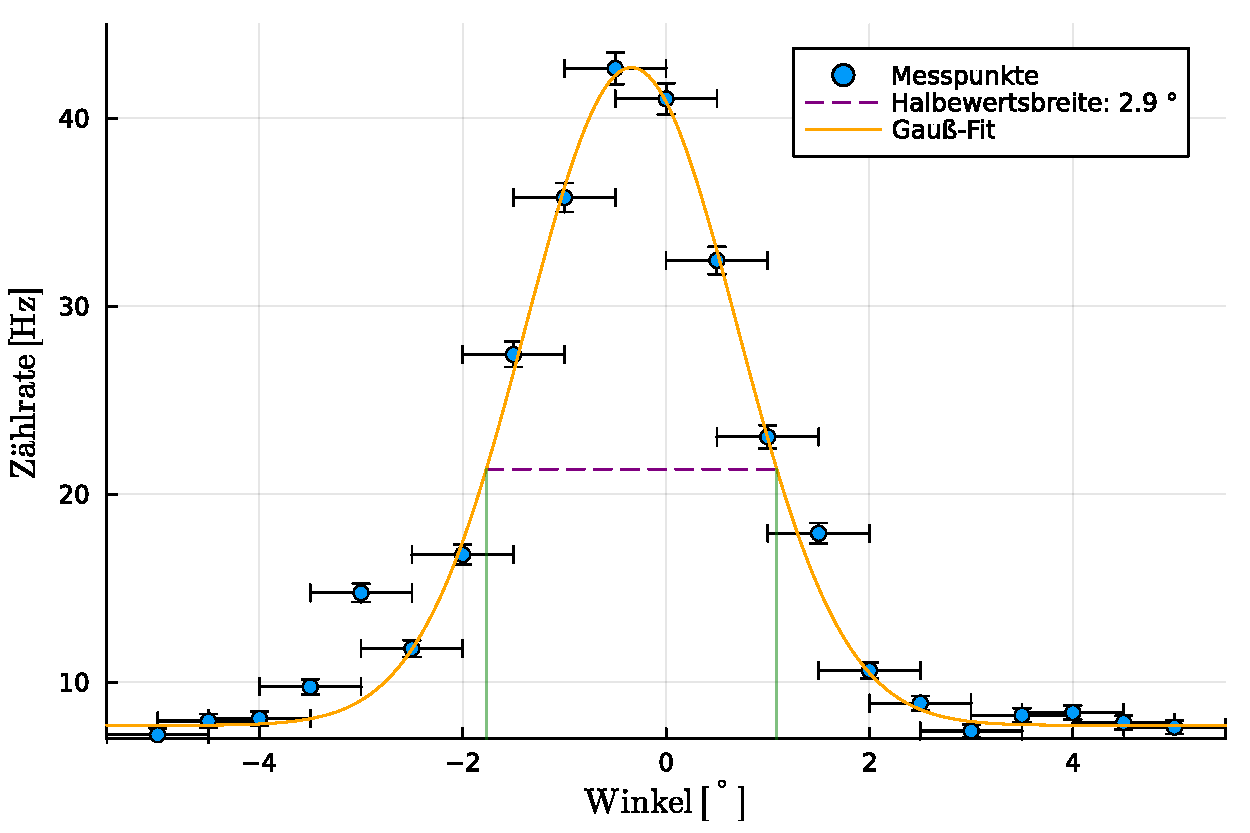
\includegraphics[width=0.9\textwidth]{../media/B3.4/plot511.pdf}
	\caption{Gemessene Zählraten der zwei koinzidenten $\gamma$--Quanten aus der Paarvernichtung, bei verschiedenen Winkeln der Detektoren zueinander (blau), mit Gaußkurve gefittet (orange) und zugehöriger Halbwertsbreite (lila)}
	\label{fig:plot511}
\end{figure}

\begin{table}[h]
	\centering
	\begin{tabular}{c|r|r||c|r|r}
		$\theta\ [^\circ]$ & $n(\theta)\ [\frac{1}{\mathrm{min}}]$ & $r(\theta)\ [\mathrm{Hz}]$ &
			$\theta\ [^\circ]$ & $n(\theta)\ [\frac{1}{\mathrm{min}}]$ & $r(\theta)\ [\mathrm{Hz}]$ \vspace{1pt}\\
		\hline 
		$-5,0 \pm 0,5$ & 432 $\pm$ 21 & 7,2 $\pm$ 0,3 &
			$5,0 \pm 0,5$ & 456 $\pm$ 21 & 7,6 $\pm$ 0,4 \\
		$-4,5 \pm 0,5$ & 476 $\pm$ 22 & 7,9 $\pm$ 0,4 &
			$4,5 \pm 0,5$ & 471 $\pm$ 22 & 7,9 $\pm$ 0,4 \\
		$-4,0 \pm 0,5$ & 484 $\pm$ 22 & 8,1 $\pm$ 0,4 &
			$4,0 \pm 0,5$ & 503 $\pm$ 22 & 8,4 $\pm$ 0,4 \\
		$-3,5 \pm 0,5$ & 585 $\pm$ 24 & 9,8 $\pm$ 0,4 &
			$3,5 \pm 0,5$ & 494 $\pm$ 22 & 8,2 $\pm$ 0,4 \\
		$-3,0 \pm 0,5$ & 885 $\pm$ 30 & 14,8 $\pm$ 0,5 &
			$3,0 \pm 0,5$ & 444 $\pm$ 21 & 7,4 $\pm$ 0,4 \\
		$-2,5 \pm 0,5$ & 707 $\pm$ 27 & 11,8 $\pm$ 0,4 &
			$2,5 \pm 0,5$ & 533 $\pm$ 23 & 8,9 $\pm$ 0,4 \\
		$-2,0 \pm 0,5$ & 1007 $\pm$ 32 & 16,8 $\pm$ 0,5 &
			$2,0 \pm 0,5$ & 637 $\pm$ 25 & 10,6 $\pm$ 0,4 \\
		$-1,5 \pm 0,5$ & 1646 $\pm$ 41 & 27,4 $\pm$ 0,7 &
			$1,5 \pm 0,5$ & 1075 $\pm$ 33 & 17,9 $\pm$ 0,5 \\
		$-1,0 \pm 0,5$ & 2147 $\pm$ 46 & 35,8 $\pm$ 0,8 &
			$1,0 \pm 0,5$ & 1383 $\pm$ 37 & 23,1 $\pm$ 0,6 \\
		$-0,5 \pm 0,5$ & 2559 $\pm$ 51 & 42,7 $\pm$ 0,8 &
			$0,5 \pm 0,5$ & 1946 $\pm$ 44 & 32,4 $\pm$ 0,7 \\
		$\pm 0,0 \pm 0,5$ & 2462 $\pm$ 50 & 41,0 $\pm$ 0,8 &---&---$\quad\ \ $&---\hspace{7mm}
	\end{tabular}
	\caption{Gemessene Ereignisse und daraus bestimmte Zählraten der Koinzidenzmessung der zwei $\gamma$-Quanten aus der Paarvernichtung}
	\label{table:messwerte511}
\end{table}

Dies entspricht unseren Erwartungen. Damit zwei $\gamma$--Quanten mit Detektoren, deren Winkel kleiner als $180\,^\circ$ zueinander ist, koinzident gemessen werden, musste das Positron oder das Elektron bei der Paarvernichtung noch einen Restimpuls gehabt haben. Dies ist jedoch aufgrund der hohen Energieabhängigkeit des Wirkungsquerschnittes bei der Paarvernichtung deutlich unwahrscheinlicher als eine Paarvernichtung bei ruhendem Positron und Elektron.\footnote{Vergleiche Abschnitt \ref{paarvernichtung}} Daher wurden nur wenige Ergebnisse bei einem Messwinkel $\theta\neq 0\,^\circ$ erwartet.

Diese Gaußverteilung mit einem Peak bei ca. $0\,^\circ$ rührt daher, dass für steigende Winkel auch der benötigte Restimpuls zunimmt. Es wird also stetig unwahrscheinlicher, ein koinzidentes Ereignis zu messen, je weiter man von $0^\circ$ abweicht.

Des weiteren ist es möglich, dass die $\gamma$--Quanten auf dem Weg zu den Detektoren abgelenkt werden und so Ereignisse auch bei Winkeln $\theta\neq 0^\circ$ aufgezeichnet werden können, bei denen sich das Positron und das Elektron bei der Paarvernichtung in Ruhe befunden haben. Dieses Phänomen sollte allerdings nur wenige Ereignisse ermöglichen und lässt uns so trotzdem eine normalverteilte Winkelverteilung erwarten.

Mittels der Gaußkurve lässt sich nun die Halbwertsbreite $\alpha_{1/2}$ der Messung bestimmen. Diese folgt aus der Standardabweichung $\sigma$ und ergibt sich zu ca. $2,4 \mathrm{\, ^\circ}$.

\begin{eqnarray}
	\alpha_{1/2} = 2 \sqrt{2 \ln 2} \cdot \sigma
\end{eqnarray}

\subsubsection{Koinzidenter Zerfall}
Zuletzt wird die Winkelabhängigkeit aus der Detektion eines $\gamma$--Quants der Paarvernichtung und eines koinzident erzeugten $\gamma$--Quants, das aus dem sekundären Zerfall von $\ce{^{22}Ne}$ in den Grundzustand stammt, untersucht. Da dies zwei koinzidente, aber unabhängige Ereignisse sind, wird keine Winkelabhängigkeit erwartet.

Analog zu Abschnitt \ref{auswertung-paarvernichtung} werden die Zählraten ermittelt und gegen den Messwinkel $\theta$ aufgetragen. Die Ergebnisse sind in Abbildung \ref{fig:plot1275} und Tabelle \ref{table:messwerte1275} dargestellt. Weiterhin wurde der Mittelwert $\bar r\approx 0,45\,\mathrm{Hz}$ der gemessenen Werte als konstante Linie eingetragen. Etwa die Hälfte der Messwerte liegen im Rahmen ihrer Ungenauigkeit um den Mittelwert $\bar r$ verteilt, die meisten der anderen Messwerte treffen bei Verdopplung ihres Fehlers den Mittelwert.

Auch dies entspricht unseren Erwartungen. Da der $\gamma$--Quant aus dem Zerfall von $\ce{^{22}Ne}$ in den Grundzustand isotrop abgestrahlt wird, sollte eine koinzidente Messung mit einem $\gamma$--Quant aus der Paarvernichtung für alle Winkel etwa gleich häufig auftreten.

Weiterhin ist die Zählrate bei dieser Messung für alle Winkel deutlich kleiner als bei der koinzidenten Messung der zwei $\gamma$--Quanten aus der Paarvernichtung. Das lässt sich ebenso damit erklären, dass das $\gamma$--Quant aus dem Zerfall von $\ce{^{22}Ne}$ in den Grundzustand isotrop abgestrahlt wird. Eine koinzidente Messung dieses $\gamma$--Quants mit einem $\gamma$--Quant aus der Paarvernichtung, sollte also deutlich seltener stattfinden, da es nur in den wenigsten Fällen, überhaupt in die Richtung des Detektors ausgesendet wird.

Größenordnungstechnisch lässt sich dies unter der Annahme abschätzen, dass der Detektor einen deutlich kleineren Radius besitzt, als sein Abstand zur Probe beträgt. Sei der Radius des Detektors beispielsweise $1 \mathrm{\, cm}$ und sein Abstand zur Probe $10 \mathrm{\, cm}$.

Damit ergeben sich die Fläche des Detektors $A_\mathrm{Det}$ sowie die Kugeloberfläche des Raumes $O_\mathrm{Raum}$, in den die Probe abstrahlt. Der Anteil $p_\gamma$ an abgestrahlten $\gamma$--Quanten, die auf den Detektor treffen, ist als das Verhältnis dieser Flächen gegeben.

\begin{eqnarray}
	A_\mathrm{Det} &=& \pi r^2 \\
	O_\mathrm{Raum} &=& 4 \pi r^2 \\
	p_\gamma &=& \frac{A_\mathrm{Det}}{O_\mathrm{Raum}} \\
	\Rightarrow \qquad p_\gamma &\approx& 0,01
\end{eqnarray}

\noindent
Nur ca. $1 \mathrm{\, \%}$ der ausgesendet $\gamma$--Quanten treffen in diesem Beispiel auf den Detektor, wodurch eine ca. 100--fach kleinere Zählrate als in der vorherigen Messung erwartet wird.

\begin{figure}[h]
	\centering
	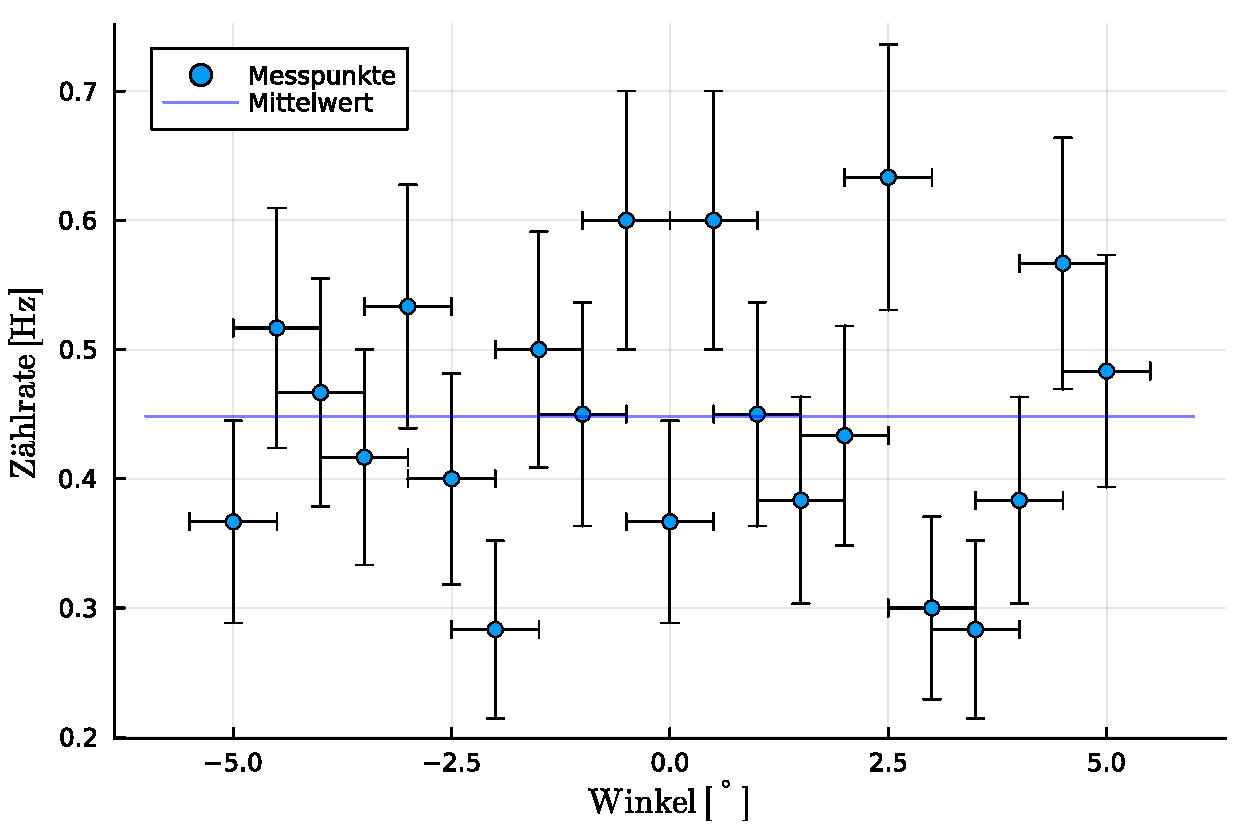
\includegraphics[width=0.9\textwidth]{../media/B3.4/plot1275.pdf}
	\caption{Gemessene Zählraten von Koinzidenzen zwischen einem $\gamma$--Quant aus der Paarvernichtung und einem $\gamma$--Quant aus dem Zerfall von $^{22}$Ne in den Grundzustand, bei verschiedenen Winkeln der Detektoren zueinander, zusammen mit dem Mittelwert (blaue Linie)}
	\label{fig:plot1275}
\end{figure}

\begin{table}[h!]
	\centering
	\begin{tabular}{c|c|c||c|c|c}
		$\theta\ [^\circ]$ & $n(\theta)\ [\frac{1}{\mathrm{min}}]$ & $r(\theta)\ [\mathrm{Hz}]$ &
			$\theta\ [^\circ]$ & $n(\theta)\ [\frac{1}{\mathrm{min}}]$ & $r(\theta)\ [\mathrm{Hz}]$ \vspace{1pt}\\
		\hline 
		$-5,0 \pm 0,5$ & 22 $\pm$ 5 & 0,37 $\pm$ 0,08 &
			$5,0 \pm 0,5$ & 29 $\pm$ 5 & 0,48 $\pm$ 0,09 \\
		$-4,5 \pm 0,5$ & 31 $\pm$ 6 & 0,52 $\pm$ 0,09 &
			$4,5 \pm 0,5$ & 34 $\pm$ 6 & 0,57 $\pm$ 0,10 \\
		$-4,0 \pm 0,5$ & 28 $\pm$ 5 & 0,47 $\pm$ 0,09 &
			$4,0 \pm 0,5$ & 23 $\pm$ 5 & 0,38 $\pm$ 0,08 \\
		$-3,5 \pm 0,5$ & 25 $\pm$ 5 & 0,42 $\pm$ 0,08 &
			$3,5 \pm 0,5$ & 17 $\pm$ 4 & 0,28 $\pm$ 0,07 \\
		$-3,0 \pm 0,5$ & 32 $\pm$ 6 & 0,53 $\pm$ 0,09 &
			$3,0 \pm 0,5$ & 18 $\pm$ 4 & 0,30 $\pm$ 0,07 \\
		$-2,5 \pm 0,5$ & 24 $\pm$ 5 & 0,40 $\pm$ 0,08 &
			$2,5 \pm 0,5$ & 38 $\pm$ 6 & 0,63 $\pm$ 0,10 \\
		$-2,0 \pm 0,5$ & 17 $\pm$ 4 & 0,28 $\pm$ 0,07 &
			$2,0 \pm 0,5$ & 26 $\pm$ 5 & 0,43 $\pm$ 0,08 \\
		$-1,5 \pm 0,5$ & 30 $\pm$ 5 & 0,50 $\pm$ 0,09 &
			$1,5 \pm 0,5$ & 23 $\pm$ 5 & 0,38 $\pm$ 0,08 \\
		$-1,0 \pm 0,5$ & 27 $\pm$ 5 & 0,45 $\pm$ 0,09 &
			$1,0 \pm 0,5$ & 27 $\pm$ 5 & 0,45 $\pm$ 0,09 \\
		$-0,5 \pm 0,5$ & 36 $\pm$ 6 & 0,60 $\pm$ 0,10 &
			$0,5 \pm 0,5$ & 36 $\pm$ 6 & 0,60 $\pm$ 0,10 \\
		$\pm 0,0 \pm 0,5$ & 22 $\pm$ 5 & 0,37 $\pm$ 0,08 &---&---&---
	\end{tabular}
	\caption{Gemessene Ereignisse und daraus bestimmte Zählraten der Koinzidenzmessung eines $\gamma$--Quanten aus der Paarvernichtung und eines $\gamma$--Quanten aus dem Zerfall von $\ce{^{22}Ne}$ in den Grundzustand}
	\label{table:messwerte1275}
\end{table}

\clearpage
\hypertarget{fazit}{%
\section{Fazit}\label{fazit}}
Die Experimente sind größtenteils sehr zufriedenstellend verlaufen. Die Untersuchung der einzelnen Signale sowie die der Winkelabhängigkeiten entsprechen den Erwartungen. Die Ortsauflösung ist ebenfalls sehr gut und im Rahmen der angenommenen Messungenauigkeit sogar vernachlässigbar.

Insbesondere bedeutet dies, dass die Auflösung sehr viel besser als die Abstände zwischen zwei Positionen sind, die für den PET--Scan der verschlossenen Truhe verwendet wurden. In allen gemessenen Richtungen kann man davon ausgehen, dass die Ortsauflösung keinen nennenswerten Einfluss auf die Messergebnisse dieses PET--Scans hat.

Auch der PET--Scan selbst ist ziemlich gut verlaufen. Es gibt für zwei Proben sehr eindeutige Ergebnisse, die in Abbildung \ref{abb:heatmap} erneut dargestellt sind. Nur die dritte Probe konnte nicht gemessen werden. Dies liegt sehr wahrscheinlich daran, dass sie um einen Faktor von über $80$ schwächer als die anderen beiden Proben ist. Damit wird ihre Strahlung in unseren Messrichtungen von den anderen beiden Proben so sehr überlagert, dass sie praktisch nicht zu erkennen ist.

Abhilfe hierfür hätte eine weitere Messreihe geben können, bei denen eine $z^\prime$--Richtung vermessen wird, die senkrecht zu der von uns verwendeten $z$--Richtung steht. Die besten Ergebnisse würden möglicherweise Messungen in $x$--, $y$--, $z$-- und $z^\prime$--Richtung liefern.

\begin{figure}[h]
	\centering
	\vspace{24pt}
	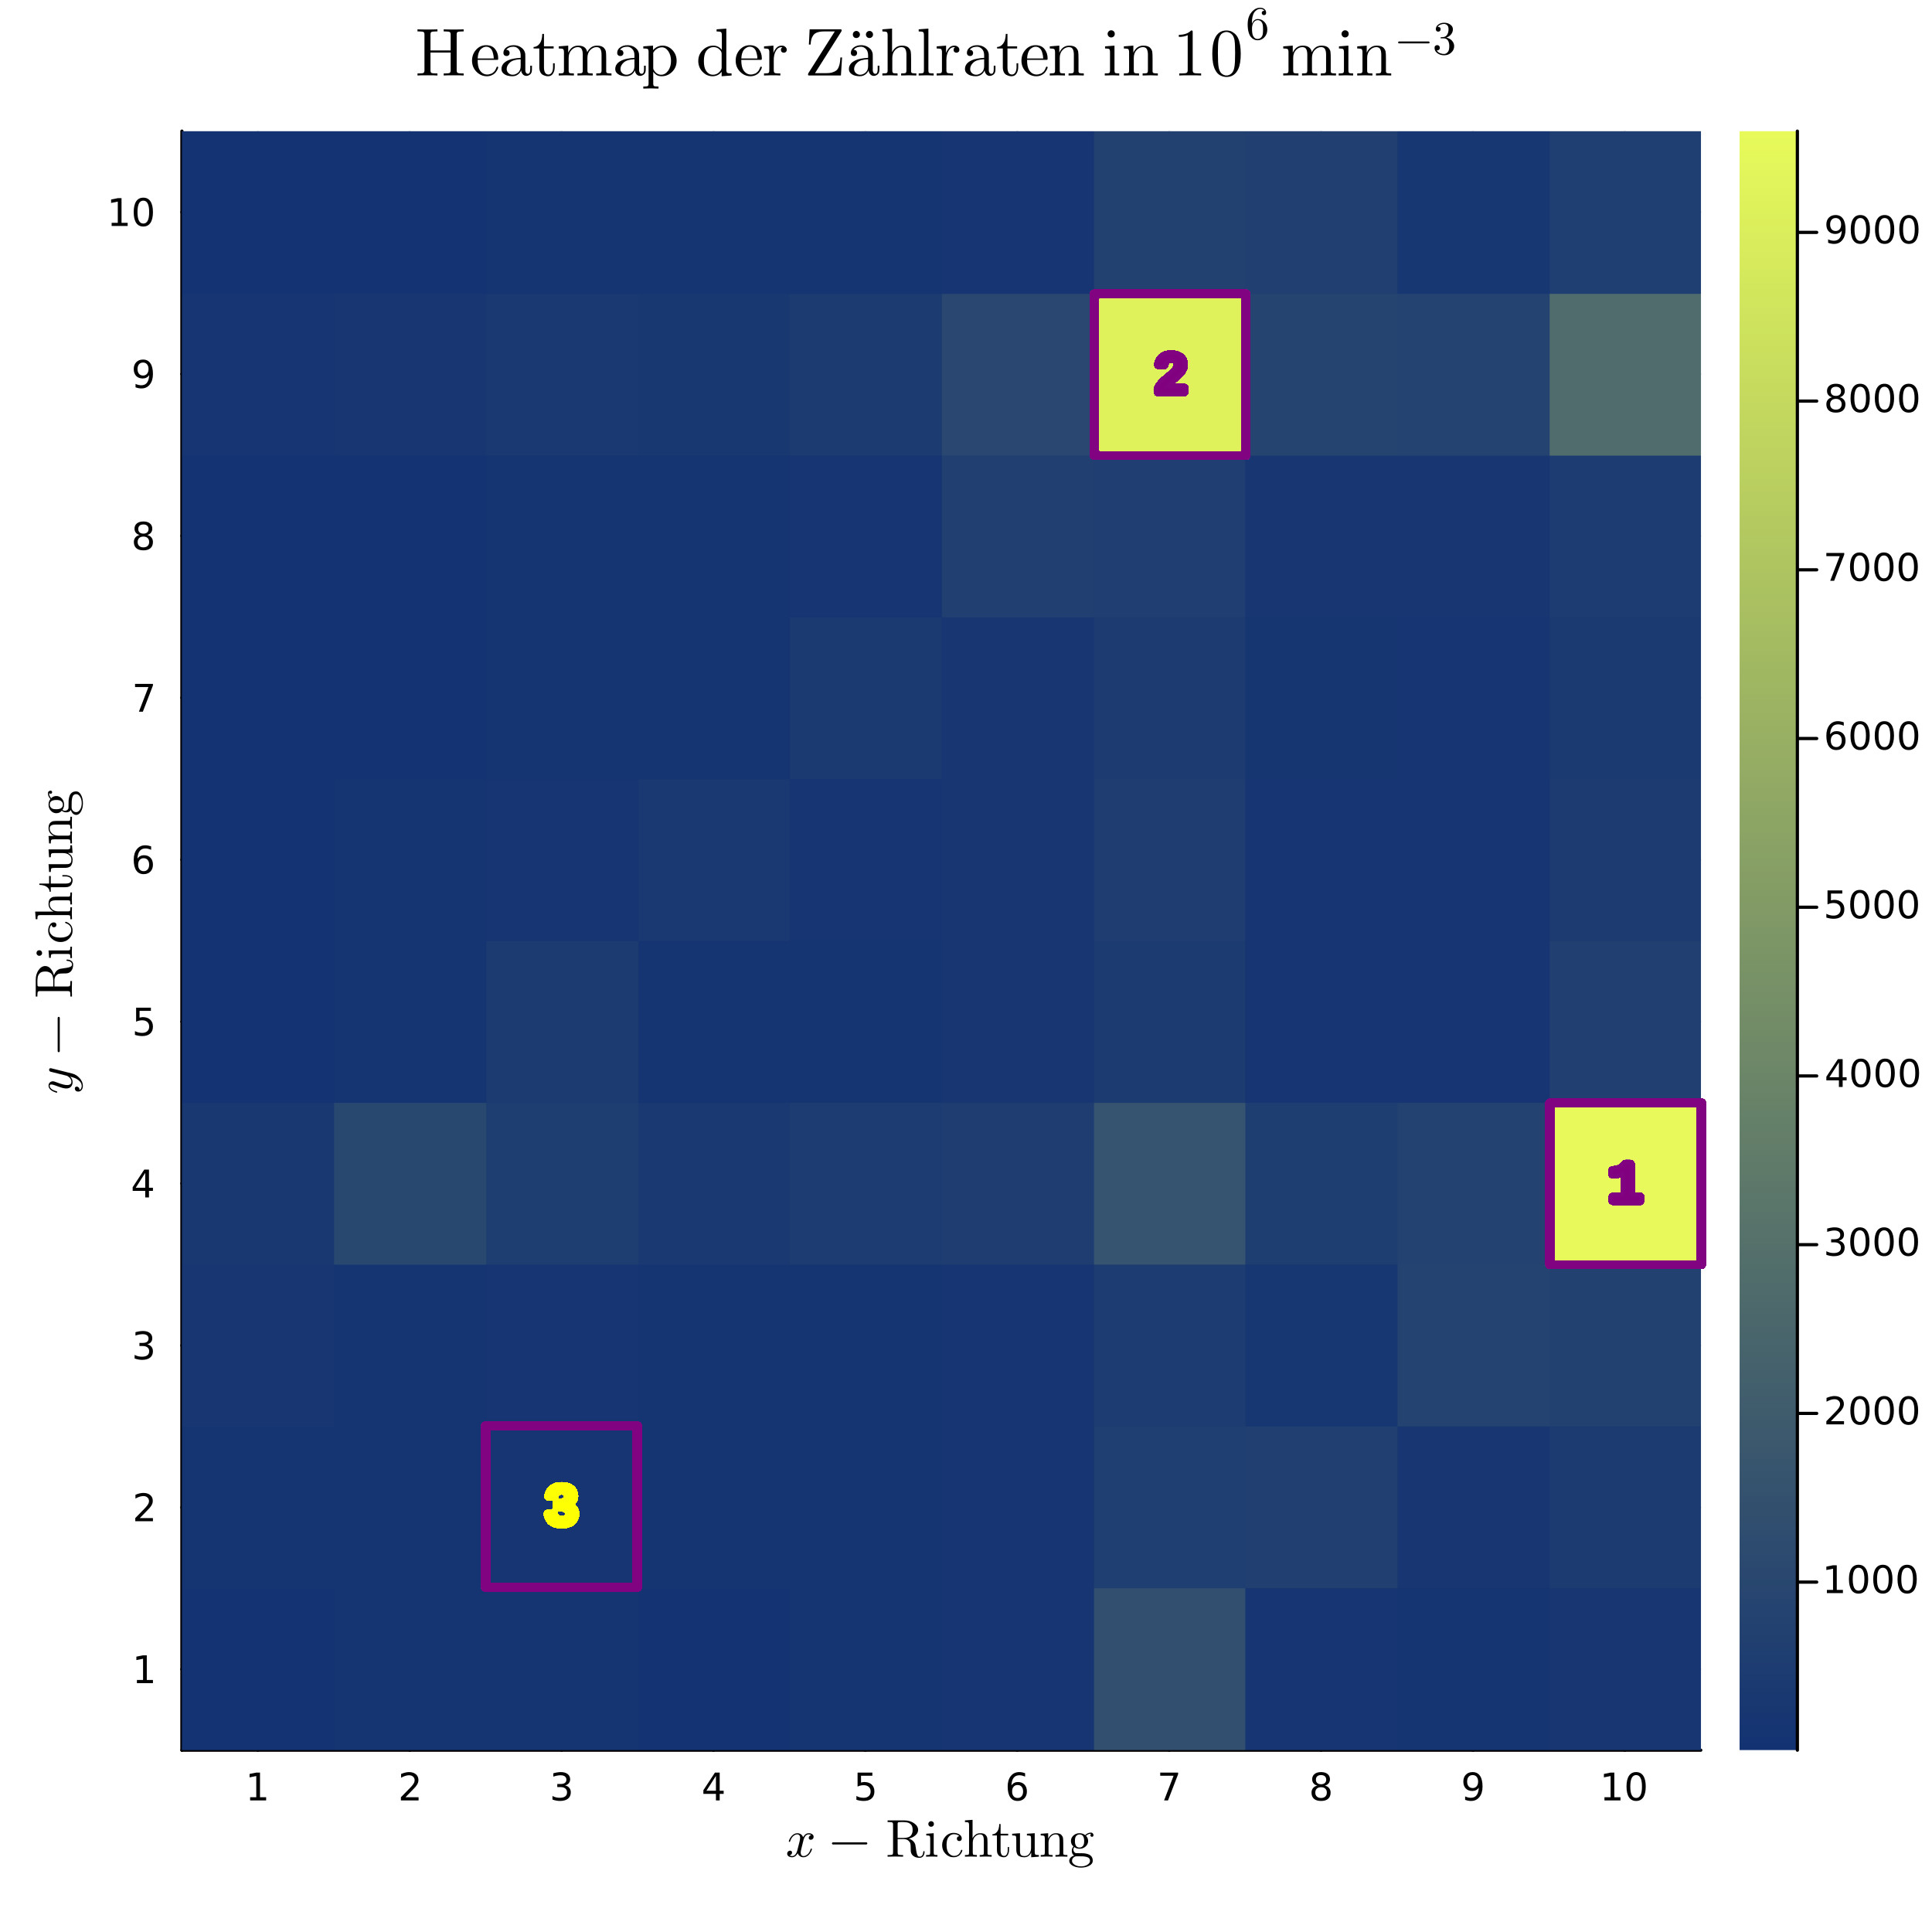
\includegraphics[width=0.6\textwidth]{../media/B3.4/heatmap.jpg}
	\caption{$z$--Richtung läuft diagonal von oben links nach unten rechts, \\
		$z^\prime$--Richtung liefe diagonal von unten links nach oben rechts}
	\label{abb:heatmap}
\end{figure}

\clearpage
\hypertarget{literatur}{\section{Literaturverzeichnis}\label{literatur}}
\renewcommand{\section}[2]{}

\begin{thebibliography}{99}
\bibitem{Bethge}
	K. Bethge, ``Kernphysik: Eine Einführung'', 3. aktualisierte und
	erweiterte Auflage, Springer--Verlag, 2008, DOI:
	\href{https://doi.org/10.1007/978-3-540-74567-9}{10.1007/978-3-540-74567-9}
\bibitem{Demtröder}
	W. Demtröder, ``Experimentalphysik 4: Kern-, Teilchen- und
	Astrophysik'', Springer--Spektrum--Verlag, 2017, DOI:
	\href{https://link.springer.com/book/10.1007/978-3-662-52884-6}{10.1007/978-3-662-52884-6}
\bibitem{NuclideChart}
	National Nuclear Data Center, ``Chart of Nuclides'',
	\url{https://www.nndc.bnl.gov/nudat3}, Abruf am 28.03.2024
\bibitem{DGNM}
	Deutsche Gesellschaft für Nuklearmedizin e.V., ``PET'',
	Online verfügbar unter
	\url{http://www.nuklearmedizin.de/docs/pet_bro_06.pdf},
	Abruf am 03.04.2024
\bibitem{Paarvernichtung}
	Lexikon der Physik, ``Paarvernichtung'',
	\url{https://www.spektrum.de/lexikon/physik/paarvernichtung/10838},
	Abruf am 04.04.2024
\bibitem{SSK}
	Strahlenschutzkommission, ``Orientierungshilfe SSK'', 2006, ISBN 3873441306,
	\url{https://campus-nes.de/fileadmin/user_upload/Orientierungshilfe_SSK.pdf}, Abruf am 07.04.2024
\bibitem{Impulshöhenspektrum}
	Lexikon der Physik, ``Impulshöhenspektrum'',
	\url{https://www.spektrum.de/lexikon/physik/impulshoehenspektrum/7156},
	Abruf am 08.04.2024
\bibitem{Escapelinie}
	Lexikon der Physik, ``Gammaspektrum'',
	\url{https://www.spektrum.de/lexikon/physik/gammaspektrum/5517},
	Abruf am 08.04.2024
\bibitem{LMU}
	LMU München, ``Detektor'',
	\url{https://homepages.physik.uni-muenchen.de/~Otmar.Biebel/detektor/detector06.pdf},
	Abruf am 07.04.2024
\bibitem{EigenschaftenSzintillatoren}
	ResearchGate, ``Daten einiger Szintillatoren'',
	\url{https://www.researchgate.net/file.PostFileLoader.html?id=54b69483d4c11860268b480d&assetKey=AS%3A273689545773057%401442264081272},
	Abruf am 10.05.2024
\bibitem{UzK}
	Universität zu Köln, ``B3.4: PET'',
	Januar 2021,
	\url{https://www.ikp.uni-koeln.de/fileadmin/data/praktikum/B3.4\_PET\_de.pdf},
	Abruf am 20.03.2024
\bibitem{Annihilation}
	Wikipedia, ``Annihilation'',
	\url{https://de.wikipedia.org/wiki/Annihilation}, Abruf am 04.04.2024
\bibitem{abb:Compton}
	Wikipedia,
	\url{https://de.wikipedia.org/wiki/Datei:Compton-spektrum.svg},
	Abruf am 08.04.2024
\bibitem{abb:Spektrum}
	Wikipedia,
	\url{https://de.wikipedia.org/wiki/Datei:Am-Be-SourceSpectrum.jpg},
	Abruf am 08.04.2024
\bibitem{abb:Photomultiplier}
	Wikipedia,
	\url{https://de.wikipedia.org/wiki/Datei:Photomultiplier_schema_de.png},
	Abruf am 08.04.2024
\bibitem{abb:Constant_fraction}
	Wikipedia,
	\url{https://commons.wikimedia.org/wiki/File:Constant_fraction_1.svg},
	Abruf am 06.04.2024
\bibitem{abb:CDF}
	Wikipedia,
	\url{https://commons.wikimedia.org/wiki/File:CFD_Diagram1.jpg},
	Abruf am 06.04.2024
\bibitem{abb:Wirkungsquerschnitte}
	Wikipedia, ``File:Pb-gamma-xs.svg'',
	\url{https://commons.wikimedia.org/wiki/File:Pb-gamma-xs.svg}, Abruf am 12.05.2024
\end{thebibliography}
\end{document}
